%!TEX root = ../main.tex

\pmax{Think story!}

We describe our novel symbolic execution engine for \jsil, an intermediate
representation for JavaScript analysis previously introduced by \citet{javert}. 
In \S\ref{subsec:jsil:analysis:formalism}, we define an abstract semantics for 
\jsil, which we then instantiate to obtain its concrete and symbolic semantics.
In \S\ref{sex:formal:guarantees}, we present the formal guarantees of 
our symbolic analysis, including: \dtag{i} a soundness result for the \jsil symbolic 
execution, \dtag{ii} a guarantee of absence of false positives for bug-finding, \pmaxinline{Do we know what bug-finding is here?}
\dtag{iii} a justification result for the lifting of analyses on compiled \jsil code back to JavaScript;
and \dtag{iv} \polish{a verification result that precisely states the conditions 
under which symbolic execution gives us verification guarantees.}
Finally, in \S\ref{subsec:jsil:analysis:implementation}, we give a brief overview
of our implementation. %in \rosette~\cite{Rosette1,Rosette2} NO NO NO! Burn the witch!


\subsection{Syntax and Semantics}\label{subsec:jsil:analysis:formalism}

\subsubsection{Syntax} 
\jsil is a simple goto language featuring top-level procedures and commands operating on object heaps. It was purposefully designed to natively support the main dynamic features of JavaScript: extensible objects; dynamic property access; and dynamic procedure calls. The syntax of \jsil is shown below. 

\vspace{5pt}
\begin{display}{Syntax of the \jsil Language}{
\begin{tabular}{llllll}
	 Numbers: $\jnumber \in \numbers$ &  Booleans: $\jbool \in \bools$ & \  \ Strings: $\jstring \in \strings$ & \  \ Locations: $\loc \in \locs$ & \  Vars: $\jvar \in \jvars$ & \ Types: $\jtype \in \jtypes$ \\[0.1cm]
\multicolumn{6}{l}{Values: $\val \in \vals$ \defeq \ $\jnumber \! \mid \! \jbool \! \mid \! \jstring \! \mid \! \jundefined \! \mid \! \jnull \! \mid \! \jempty \! \mid \! \loc \! \mid \! \jtype \! \mid \!  \pid$ \qquad Expressions: $\jsilexpr \in \exprs$ \defeq \ $\val \mid \jvar \mid \ominus\ \jsilexpr \mid \jsilexpr \binop{} \jsilexpr $} \\[0.1cm]
	\multicolumn{6}{l}{Basic Commands: $\bcmd \in \bcmds$ \defeq\ $\jsilskip \mid \jvar := \jsilexpr  \mid \jvar := \jsilnew() \mid \jvar := [\jsilexpr, \jsilexpr] \mid [\jsilexpr, \jsilexpr] := \jsilexpr \mid$} \\[0.1cm]
	\multicolumn{6}{l}{\hspace{3.29cm} $\jsildelete(\jsilexpr, \jsilexpr) \mid \jvar := \hasfield(\jsilexpr, \jsilexpr) \mid \jvar := \getfields(\jsilexpr) \mid \jvar := \makesymbolic(\jtype)$} \\[0.1cm]
	% Commands
	\multicolumn{6}{l}{Commands: $\jcmd \in \cmds$ \defeq \ $ \bcmd \mid \goto \ i \mid  \ifgoto{\jsilexpr}{i}{j} \mid \jsilcall{\jvar}{\jsilexpr}{\jvec{\jsilexpr}}{j} 
	         \mid \assume(\jsilexpr) \mid \assert(\jsilexpr)$} \\[0.1cm]
	\multicolumn{6}{l}{Procedures : $\proc \in \procs$ \defeq \ $\procedure{\pid}{\jvec{\jvar}}{\jvec{\jcmd}}$}
 \end{tabular}}
\end{display}

\vspace{5pt}
\noindent \jsil \emph{values}, $\val \in \vals$, include numbers, booleans, strings, the special values $\jundefined$, $\jnull$, and $\jempty$, as well as types~$\jtype$, and procedure identifiers $\pid$.
\jsil~\emph{expressions}, $\jsilexpr \in \exprs$, include \jsil values, \jsil program variables $\jvar$, and various unary and binary operators, which, for instance, provide support for sets and lists. 

\jsil \emph{basic commands} enable the manipulation of extensible objects and do not affect control flow. 
They include $\jsilskip$, variable assignment, object creation, property access, property assignment, property deletion, membership check,  property collection, and symbolic variable creation. 

\jsil \emph{commands} include \jsil basic commands and commands related to control flow: conditional and unconditional gotos, dynamic procedure calls, and two special commands, $\assume$ and $\assert$, essential for symbolic execution, but with trivial concrete semantics.\footnote{\jsil also has a $\phi$-node assignment, which allows \JSComp to produce code directly in Static-Single-Assignment (SSA) \cite{SSA}. To avoid clutter, we omit the $\phi$-node assignment from the formal presentation as it does not impact the reasoning. Details can be found in \cite{javert}.} 
The two goto commands are straightforward: $\goto \ i$ jumps to the $i$-th command of the active procedure, and $\ifgoto{\jsilexpr}{i}{j}$ jumps to the $i$-th command if $\jsilexpr$ evaluates to $\jtrue$, and to the $j$-th if it evaluates to $\jfalse$. 
The dynamic procedure call $\jsilcall{\jvar}{\jsilexpr}{\jvec{\jsilexpr}}{j}$ first evaluates  $\jsilexpr$ and $\jvec{\jsilexpr}$ to obtain the procedure identifier and arguments, respectively, executes the appropriate procedure with these arguments, and, in the end, assigns its return value to $\jvar$.
If the procedure raises an error, control is transferred to the $j$-th command; otherwise, it simply follows to the next command. 

A \jsil program $\prog \in \progs$ can be seen as a set of top-level procedures of the form $\procedure{\pid}{\jvec{\jvar}}{\jvec{\jcmd}}$, where $\pid$ is the procedure identifier, $\jvec{\jvar}$ are its formal parameters, and its body ${\jvec{\jcmd}}$  is a sequence of \jsil commands.
Every \jsil program contains a special procedure $\jsilmain$\hspace{-2pt}, denoting the entry point of the program. 
\jsil procedures return via two dedicated indexes, $\retlab$ and $\errlab$, using two dedicated variables, $\retvar$ and $\errvar$. If a procedure reaches the $\retlab$ index, it returns normally with the return value denoted by $\retvar$; when it reaches $\errlab$, it returns an error, with the error value denoted by $\errvar$.

%

\subsubsection{Abstract Semantics}
We first define an abstract semantics for \jsil, which is parametric on a \jsil \emph{state signature}. 
Then, we instantiate this abstract semantics with a concrete state signature to obtain the \emph{concrete semantics} for \jsil, and with a symbolic state signature to obtain its symbolic counterpart.
This approach to the design of symbolic analyses has the following main benefits: \dtag{1} it streamlines the formalism, avoiding redundancy,
\dtag{2} it makes explicit the choices in the design of the symbolic semantics,
and \dtag{3} it leads to modular implementations, avoiding code duplication.


The abstract semantics is parametric on abstract states $\absstate \in \absstates$ and abstract values $\absval \in \absvals$.
Abstract states are assumed to have a store component $\absstore: \jvars \partialmap \absvals$, mapping program variables $\jvar \in \jvars$ to abstract values. Abstract values must include: \jsil values, $\val$; abstract locations, $\absloc$; abstract property names, $\absprop$; sets of abstract values; and the special value $\none$, used to indicate the absence of a property in an object. Abstract states expose the following functions and relations: 
\begin{description}
\setlength{\itemsep}{0.2em}
  \item[\jsil Expression Evaluation,] $\evalexpr{} :  (\jvars \partialmap \absvals)  \partialmap \exprs \partialmap \absvals$. 
  	The expression $\evalexpr{}(\absstore, \jsilexpr)$ evaluates to the abstract value of the \jsil expression $\jsilexpr$ under store $\absstore$. 
            
  \item[Store Selector,] $\stosel : \absstates \rightarrow (\jvars \partialmap \absvals)$. The expression $\stosel(\absstate)$ evaluates to the abstract store associated with a given abstract state $\absstate$. For clarity, we write $\absstate.\stosel$ instead of $\stosel(\absstate)$. 
             
  \item[Store Update,] $\stupdt{}: \absstates \rightarrow \jvars \rightarrow \absvals \rightarrow \absstates$. 
             The expression $\stupdt{}(\absstate, \jvar, \absval)$ denotes the abstract state obtained from $\absstate$ 
             by updating the abstract value corresponding to $\jvar$ in $\absstate.\stosel$ to $\absval$. 

   \item[Heap Update,] $\hpupdt{} : \absstates \rightarrow \absvals \partialmap \absvals \partialmap \absvals \partialmap \absstates$. 
             The expression $\hpupdt{}(\absstate, \absloc, \absprop, \absval)$ denotes the abstract state obtained from $\absstate$ 
             by updating the value of property $\absprop$ of the object at location $\absloc$ to $\absval$. 
                   
  
  \item[GetCell,] $\getcell \subseteq \absstates \times \exprs \times \exprs \times \absstates \times \absvals \times \absvals \times \absvals$. 
          We pretty-print $(\absstate, \jsilexpr_1, \jsilexpr_2, \absstate', \absloc, \absprop, \absval) \in \getcell$ as $\absgetcellrule{}{\absstate, \jsilexpr_1, \jsilexpr_2}{\absstate', (\absloc, \absprop, \absval)}$. 
          Informally, GetCell retrieves the value associated with a given property of a given object. More formally, if $\absgetcellrule{}{\absstate, \jsilexpr_1, \jsilexpr_2}{\absstate', (\absloc, \absprop, \absval)}$ holds, 
          then \dtag{1} $\absloc$ denotes the abstract location resulting from the evaluation of $\jsilexpr_1$, 
          \dtag{2} $\absprop$ denotes the abstract property name resulting from the evaluation of $\jsilexpr_2$, 
          \dtag{3} $\absval$ denotes the abstract value of the property $\absprop$ of the object at location $\absloc$, 
          and \dtag{4} $\absstate'$ denotes a (potential) modification of $\absstate$ that allows for the property inspection (discussed shortly). 
          Note that $\getcell$ is non-deterministic and is, therefore, a relation.
             
  \item[GetDomain,] $\getdomain \subseteq \absstates \rightarrow \exprs \partialmap \absvals$. 
           We pretty-print $(\absstate, \jsilexpr, \absval) \in \getdomain$ as $\absgetdomainrule{}{\absstate, \jsilexpr}{\absval}$. 
           If $\absgetdomainrule{}{\absstate, \jsilexpr}{\absval}$ holds, then $\absval$ denotes the 
           set of abstract property names associated with the object at the location resulting from the evaluation of $\jsilexpr$ 
           in $\absstate$. 
   
   \item[Assumption,] $\absassume{} : \absstates \rightarrow \exprs \partialmap \absvals$. 
            The expression $\absassume{}(\absstate, \jsilexpr)$ denotes the abstract state obtained from the 
            abstract state $\absstate$ by assuming that $\jsilexpr$ evaluates to the boolean $\jtrue$. 
  
   \item[Satisfiability,] $\abssat{} : \absstates \rightarrow \exprs \partialmap \bools$. 
            The expression $\abssat{}(\absstate, \jsilexpr)$ evaluates to $\jtrue$ if the \jsil expression $\jsilexpr$ is \polish{satisfiable} in the abstract 
            state $\absstate$, and $\jfalse$ otherwise.
             
   \item[Symbolic Value Creation,] $\absmakesymbolic : \jtypes \rightarrow \absvals$. 
            The expression $\absmakesymbolicrule{}{\jtype}$ evaluates to a fresh symbolic value of type $\jtype$.
\end{description}

\begin{figure}[ht!]
{\scriptsize
\begin{mathpar}
  \inferrule[\textsc{Skip}]{}
	{ \absbsemrule{\absstate, \jsilskip}{\absstate}{}}  	
\and 
\inferrule[\textsc{Property Collection}]
  {
           \absgetdomainrule{}{\absstate, \jsilexpr}{\absval}  
  }{\absbsemrule{\absstate, \jvar := \getfields(\jsilexpr)}{\stupdt{}(\absstate, \jvar, \absval)}{}} 
\and 
\inferrule[\textsc{Assignment}]
  {
        \absstore = \absstate.\stosel
        \quad 
        \absval = \evalexpr{}(\absstore, \jsilexpr)
  }{\absbsemrule{\absstate, \jvar := \jsilexpr}{\stupdt{}(\absstate, \jvar, \absval)}{}} 
\\
\inferrule[\textsc{Object Creation}]
  { 
   \loc \text{ fresh}
  }{\absbsemrule{\absstate, \jvar := \jsilnew()}{\hpupdt{}(\absstate, \loc, \protop, \jnull)}{}}
\and 
\inferrule[\textsc{Property Access}]
  { 
  	\absgetcellrule{}{\absstate, \jsilexpr_1, \jsilexpr_2}{\absstate', (-, -, \absval)}
  }{ \absbsemrule{\absstate, \jvar := [\jsilexpr_1, \jsilexpr_2]}{\stupdt{}(\absstate', \jvar, \absval)}{}}
%
\\
\inferrule[\textsc{Property Assignment}]
  {    
      \absgetcellrule{}{\absstate, \jsilexpr_1, \jsilexpr_2}{\absstate', (\absloc, \absprop, -)} \quad \absstore = \absstate.\stosel \quad \absval = \evalexpr{}(\absstore, \jsilexpr_3)
  }{\absbsemrule{\absstate, [\jsilexpr_1, \jsilexpr_2] := \jsilexpr_3}{\hpupdt{}(\absstate', \absloc, \absprop, \absval)}{}} 
\and
 \inferrule[\textsc{Property Deletion}]
  { 
        \absgetcellrule{}{\absstate, \jsilexpr_1, \jsilexpr_2}{\absstate', (\absloc, \absprop, \absval)}
        \quad
     	\absval \neq \none
  }{\absbsemrule{\absstate, \jsildelete(\jsilexpr_1, \jsilexpr_2)}{\hpupdt{}(\absstate', \absloc, \absprop, \none)}{}}
\\
\inferrule[\textsc{Member Check - True}]
  { 
     \absgetcellrule{}{\absstate, \jsilexpr_1, \jsilexpr_2}{\absstate', (-, -, \absval)} 
     \quad 
    \absval \neq \none
  }{\absbsemrule{\absstate, \jvar := \hasfield(\jsilexpr_1, \jsilexpr_2)}{	{}(\absstate', \jvar, \jtrue)}{}}
 \and 
\inferrule[\textsc{Member Check - False}]
  { 
     \absgetcellrule{}{\absstate, \jsilexpr_1, \jsilexpr_2}{\absstate', (-, -, \none)} 
  }{\absbsemrule{\absstate, \jvar := \hasfield(\jsilexpr_1, \jsilexpr_2)}{\stupdt{}(\absstate', \jvar, \jfalse)}{}} \\
  \inferrule[\textsc{Make Symbolic}]
  { 
     \absval = \absmakesymbolicrule{}{\jtype}
  }{\absbsemrule{\absstate, \jvar := \makesymbolic(\jtype)}{\stupdt{}(\absstate, \jvar, \absval)}{}}
\end{mathpar}}
 \vspace*{-0.6cm}
\caption{Abstract Semantics for Basic Commands: {\scriptsize$\absbsemrule{\absstate, \bcmd}{\absstate'}{}$}\label{abs:sem:bcmds:fig}}
\end{figure}

\begin{figure}[ht!]
{\scriptsize
\begin{mathpar} 
\inferrule[\textsc{Basic Command}]
   { 
     \ccmd[\prog][\abscs]{i} = \bcmd 
     \\\\
     \absbsemrule{\absstate, \bcmd}{\absstate'}{} 
   }{\abssemrule{\absstate, \abscs, i}{\absstate', \abscs, i{+}1}{\top}{\top}{}}
  %
  \and
  %
  \inferrule[\textsc{Cond. Goto - True}]
   { \ccmd[\prog][\abscs]{i} =  \ifgoto{\jsilexpr}{j}{k} 
     \\\\
     %   \absval = \evalexpr{}(\absstate.\stosel, \jsilexpr)
     %   \quad 
     \absstate' = \absassume{}(\absstate, \jsilexpr) 
   }
   {\abssemrule{\absstate, \abscs, i}{\absstate', \abscs, j}{\top}{\top}{}}
  %
  \and 
  % 
  \inferrule[\textsc{Cond. Goto - False}]
   { \ccmd[\prog][\abscs]{i} =  \ifgoto{\jsilexpr}{j}{k} 
      \\\\ 
       % \absval = \evalexpr{}(\absstate.\stosel, \jsilexpr)
       % \quad 
      \absstate' = \absassume{}(\absstate, \neg\jsilexpr) 
   }
   {\abssemrule{\absstate, \abscs, i}{\absstate', \abscs, k}{\top}{\top}{}}
  %
  \\
  %
  \inferrule[\textsc{Goto}]
   { 
   \ccmd[\prog][\abscs]{i} = \goto \, j \quad}
   {\abssemrule{\absstate, \abscs, i}{\absstate, \abscs, j}{\top}{\top}{}}
   %
   \qquad 
   %
   \inferrule[\textsc{Normal Return}]
   {
       \abscs = (-, \absstore', \jvar, i, -) :: \abscs'  
       \quad 
       \absstore = \absstate.\stosel
       \\\\
       \absstate' = \absstate[\stosel \mapsto \absstore'[\jvar \mapsto \absstore(\retvar)]]
   }  
   {\abssemrule{\absstate, \abscs, \retlab}{\absstate', \abscs', i}{\top}{\top}{}}
     %
   \qquad 
   %
      \inferrule[\textsc{Error Return}]
   { 
       \abscs = (-, \absstore', \jvar, -, j) :: \abscs'
       \quad 
       \absstore = \absstate.\stosel
       \\\\
       \absstate' = \absstate[\stosel \mapsto \absstore'[\jvar \mapsto \absstore(\errvar)]]
   }  
   {\abssemrule{\absstate, \abscs, \errlab}{\absstate', \abscs', j}{\top}{\top}{}}
      \\
    \inferrule[\textsc{Procedure Call}]
   { 
    \ccmd[\prog][\abscs]{i} =   \jsilcall{\jvar}{\jsilexpr}{\jsilexpr_i \mid_{i = 0}^{n}}{j}
     \and
     \absstore = \absstate.\stosel 
     \and 
    \evalexpr{}(\absstore, \jsilexpr) =  \pid' 
        \and
     \args(\prog, \pid') = \jsillist{\jvar_1, ..., \jvar_{m}} 
      \\\\
      \absval_i = \evalexpr{}(\absstore, \jsilexpr_i) \mid_{i = 0}^{n} 
     \and
      \absval_i = \jundefined \mid_{i = n+1}^{m}  
      \and 
      \absstore' = [ \jvar_i \mapsto \absval_i \mid_{i = 0}^{m}]
      \and 
      \abscs' = (\pid', \absstore, \jvar, i{+}1, j) :: \abscs 
   }
   {\abssemrule{\absstate, \abscs, i}{\absstate[\stosel \mapsto \absstore'], \abscs', 0}{\top}{\top}{}}
    \\ 
%
\inferrule[\textsc{Assume}]
  { 
      \ccmd[\prog][\abscs]{i}  = \assume(\jsilexpr) 
      \\\\ 
      %\absstore = \absstate.\stosel
      %\quad
      %\evalexpr{}(\absstore, \jsilexpr) =  \absval
      %\\\\
     \absstate' = \absassume{}(\absstate, \jsilexpr) 
  }{\abssemrule{\absstate, \abscs, i}{\absstate', \abscs, i{+}1}{\top}{\top}{}} 
\and
\inferrule[\textsc{Assert - True}]
  { 
      \ccmd[\prog][\abscs]{i}  = \assert(\jsilexpr)
      \\\\ 
      %\absstore = \absstate.\stosel
      %\quad
      %\absval = \evalexpr{}(\absstore, \jsilexpr)
      % \\\\
       \abssat(\absstate, \neg \jsilexpr) = \jfalse
  }{\abssemrule{\absstate, \abscs, i}{\absstate, \abscs, i{+}1}{\top}{\top}{}} 
\and 
\inferrule[\textsc{Assert - False}]
  { 
      \ccmd[\prog][\abscs]{i}  = \assert(\jsilexpr)
      \\\\ 
      %\absstore = \absstate.\stosel
      %\quad
      %  \absval = \evalexpr{}(\absstore, \jsilexpr)
      % \\\\
      \abssat(\absstate, \neg \jsilexpr) = \jtrue
  }{\abssemrule{\absstate, \abscs, i}{\absstate, \abscs, i}{\top}{\bot}{}} 
 \end{mathpar}}
% \pmax{What happens when we exit from main, how do we stop? Basically, cmd returns nothing and we can't reduce?}
 \vspace*{-0.6cm}
\caption{Abstract Execution for Control Flow Commands: $\abssemrule{\absstate, \abscs, i}{\absstate', \abscs', j}{\mode}{\mode'}{}$}
\label{abs:sem:cmds:fig}
\end{figure}

Transitions for basic commands and control flow commands are given 
in Figures~\ref{abs:sem:bcmds:fig} and~\ref{abs:sem:cmds:fig}. Transitions for 
basic commands are of the form 
$\absbsemrule{\absstate, \bcmd}{\absstate'}{}$, meaning that the execution of the basic command 
$\bcmd$ in the abstract state $\absstate$ results in the abstract state $\absstate'$. 
%
To describe transitions for control flow commands, we introduce \emph{execution modes} and 
\emph{call stacks}.  \jsil has two execution modes, ranged over by $\mode$: 
$\top$, which indicates that the execution can proceed; and~$\bot$, which indicates that a failure 
has occurred and the execution must stop. Call stacks, ranged over by $\abscs$, are lists of tuples of the form $(\pid, \absstore, \jvar, i, j)$, where: 
\dtag{1}~$\pid$~is the identifier of the procedure that is currently executing;
\dtag{2}~$\absstore$~is the store of the procedure that called $\pid$; 
\dtag{3}~$\jvar$~is the variable to which the return of $\pid$ must be assigned in $\absstore$; 
\dtag{4} $i$ is the index of the command to which the control must jump after the execution of $\pid$ in case of normal return; 
and \dtag{5} $j$ is the index to which it must jump in case of error return. 
Transitions for control flow commands have the form:  $\abssemrule{\absstate, \abscs, i}{\absstate', \abscs', j}{\mode}{\mode'}{}$, 
meaning that, in the context of the entire program $\prog$, the evaluation of the $i$-th command of the first procedure in the 
call stack $\abscs$, in state $\absstate$ and execution mode $\mode$, generates 
the state $\absstate'$, call stack $\abscs$,  and the next command to be evaluated is the $j$-th command of the first procedure 
of the call stack~$\abscs'$, in execution mode $\mode'$. 
For clarity, we keep the executing program implicit and make use of a function $\ccmd{\prog, \cs, i}$, which 
returns the $i$-th command of the procedure that is first in $\cs$. %We write $\ccmd{i}$ when $\prog$ and $\ctx$ are implicit.

\jfs{
\begin{enumerate}
   \item Should we explain the rules?
   \item We shou
\end{enumerate}
}

\subsubsection{Concrete Semantics}
A \jsil concrete state $\jstate$ is a pair $(\heap, \store)$ consisting of a heap and a store. 
A heap, $\heap \in \heaps$, is a partial function mapping pairs of  object locations and property names (strings) to \polish{\jsil values},
whereas a store, $\store \in \stores$, maps \jsil program variables to \jsil values. 
Given a heap~$\heap$, we denote: the empty heap by $\hemp$; heap lookup by $\heap(\loc, \jstring)$; 
a heap cell by $\hcell{\loc}{\jstring}{\val}$, meaning that  $\heap(\loc,\jstring) = \val$; 
heap update by $\heap[(\loc, p) \mapsto \val]$, denoting the heap $\heap$ extended with $\heap(\loc,\jstring) = \val$;
and the union of two disjoint heaps by $\heap_1 \dunion \heap_2$.
We instantiate the abstract semantics for the concrete case by providing the appropriate definitions 
for the required abstract functions/relations below, noting that abstract values are instantiated to
\jsil values extended with the property absence indicator $\none$.
We write $\absbsemrule{\jstate, \bcmd}{\jstate'}{\concrete}$ for the concrete semantic 
judgement for basic commands and $\abssemrule{\jstate, \cs, i}{\jstate', \cs', j}{\mode}{\mode'}{\concrete}$ 
for control flow commands. 

\begin{display}{Concrete Semantics Rules}
\text{
{\scriptsize
\begin{mathpar} 
  \inferrule[\textsc{Expression Evaluation}]
  {}{\evalexpr{c}(\store, \val) = \val \qquad 
  	\evalexpr{c}(\store, \jvar) = \store(\jvar) \qquad 
	\evalexpr{c}(\store, \ominus \jsilexpr) = \underline{\ominus} \ \evalexpr{c}(\store, \jsilexpr) \qquad
	\evalexpr{c}(\store, \jsilexpr_1 \oplus \jsilexpr_2) = \evalexpr{c}(\store, \jsilexpr_1) \ \underline{\oplus} \ \evalexpr{c}(\store, \jsilexpr_2)}
  \\
  \inferrule[\textsc{GetDomain}]
   { 
        \evalexpr{c}(\store, \jsilexpr) = \loc
      \quad
       \heap = \heap' \, \uplus \, \big((\loc, p_i) \mapsto \val_i \big)\mid_{i = 0}^m  
      \quad
          (\loc,-) \notin \domain (\heap')  
       }{  \absgetdomainrule{\concrete}{(\heap, \store), \jsilexpr}{\jsilset{p_1, ..., p_m}}}
  %
  \and
  %
    \inferrule[\textsc{GetCell - Explicit Cell}]
   { 
         \evalexpr{c}(\store, \jsilexpr_1) = \loc
        \quad 
         \evalexpr{}(\store, \jsilexpr_2) = p
        \quad
       \heap = - \, \uplus \, (\loc, p) \mapsto \val
        }{  \absgetcellrule{\concrete}{(\heap, \store), \jsilexpr_1, \jsilexpr_2}{(\heap, \store), (\loc, p, \val)}}
 %
 \\
   \inferrule[\textsc{Store Selector}]
   {}{  \stosel((\heap, \store)) =  \store}
  	\qquad
   \inferrule[\textsc{Store Update}]
   { 
         \store' = \store[\jvar \mapsto \val]
   }{  \stupdt{\concrete}((\heap, \store), \jvar, \val) =  (\heap, \store')}
   \qquad
       \inferrule[\textsc{Heap Update - Non-$\none$}]
   { 
         \heap' = \heap[(\loc, p) \mapsto \val]
         \quad 
         \val \neq \none
   }{  \hpupdt{\concrete}((\heap, \store), \loc, p, \val) =  (\heap', \store)}
 \qquad
       \inferrule[\textsc{Heap Update - $\none$}]
   { 
         \heap = \heap' \dunion (\loc, p) \mapsto -
   }{  \hpupdt{\concrete}((\heap, \store), \loc, p, \none) =  (\heap', \store)}
  %

   \\
      \inferrule[\textsc{Assumption}]
   {}{  \absassume{\concrete}(\jstate, \jtrue) =  (\jstate, \jtrue) }
\and 
    \inferrule[\textsc{Satisfiability}]
   {}{  \abssat{\concrete}(\jstate, \jbool) = \jbool}
  \and
      \inferrule[\textsc{Symbolic Value Creation }]
   {\val \in \vals \text{ is of type } \jtype}{\absmakesymbolicrule{\concrete}{\jtype} = \val}
 \end{mathpar}
  }}
 \end{display}
  
\pmax{Perhaps a comment on the semantics - eval of expressions and something?}

\subsubsection{Symbolic Semantics}
In order to symbolically execute \jsil programs, we extend the syntax of \jsil expressions with 
symbolic strings $\sstring \in \sstrings$ and symbolic numbers $\snumber \in \snumbers$. 
For convenience, we use $\svars$ to denote the union of $\sstrings$ and $\snumbers$ 
and $\svar$ to range over $\svars$. We introduce: \jsil symbolic expressions, $\sexpr \in \sexprs$, defined as follows: $\sexpr \triangleq \val \mid \svar \mid \unoper\ \sexpr \mid \sexpr \binoper \sexpr$. 
Furthermore, we redefine \jsil expressions, $\pvsexpr \in \pvsexprs$ to take into account symbolic values
 as follows: $\pvsexpr \triangleq \val \mid \jvar \mid \svar \mid \unoper\ \pvsexpr \mid \pvsexpr \binoper \pvsexpr$.
Extended \jsil expressions differ from symbolic expressions in that they can contain program variables.
We extend heaps, stores, and call stacks with symbolic expressions, obtaining symbolic 
heaps, stores, and call stacks, respectively ranged over by $\sheap$, $\sstore$, and $\scs$.
A symbolic heap, $\sheap \in \sheaps$, is a partial function mapping pairs of  
object locations and symbolic expressions to symbolic expressions. 
A symbolic store, $\sstore \in \sstores$, is a mapping from program variables 
$\jvar \in \jvars$ to symbolic expressions. Therefore, an evaluation of a \jsil extended expression $\pvsexpr$ in a symbolic store $\sstore$ always yields a 
symbolic expression $\sexpr$.
A symbolic call stack $\scs$ only differs from a concrete call stack in that it contains 
symbolic stores instead of concrete stores.


A \emph{symbolic state} $\sstate = (\sheap, \sdom, \sstore, \pc)$ is a 4-tuple consisting of a 
symbolic heap $\sheap$, a symbolic domain $\sdom$, a symbolic store $\sstore$, and a path condition $\pc$. 
The \emph{heap domain} maps object locations to set of properties that may be defined in the corresponding object.  
The \emph{path condition}~\cite{symb:exec:survey} is a first-order quantifier-free formula over symbolic strings and 
numbers, which accumulates constraints on the given symbolic inputs that trigger 
the execution to follow the path that led to the current symbolic state.
To avoid clutter, we conflate logical values with \jsil logical values and \jsil logical 
operators with the boolean logical operators. Alternatively, we could have chosen to 
have two different types, \jsil logical expressions and logical expressions, together with a lifting 
function for converting the former to the latter. Our choice simplifies both reasoning 
and~presentation, in that a path condition is simply a \jsil symbolic expression of type boolean. 

We instantiate the abstract semantics for the symbolic case by providing the appropriate definitions 
for the required abstract functions/relations. 
We write $\absbsemrule{\jstate, \bcmd}{\jstate'}{\symbolic}$ for the symbolic semantic 
judgement for basic commands and $\abssemrule{\jstate, \cs, i}{\jstate', \cs', j}{\mode}{\mode'}{\symbolic}$ 
for control flow commands. 


\vspace{5pt}
\begin{display}{Symbolic Semantics Rules}
\text{
{\scriptsize
\begin{mathpar} 
  \inferrule[\textsc{GetDomain}]
   { 
        \evalexpr{}(\sstore, \jsilexpr) = \sloc
      \quad
       \sheap = \sheap' \, \uplus \, \big((\sloc, \sexprp_i) \mapsto \sexprv_i \big)\mid_{i = 0}^m  
        \\\\
        %
          (\sloc,-) \notin \domain (\sheap')  
        \quad
         \pc \vdash \jsilset{\sexprp_1, ..., \sexprp_m} = \sdom(\sloc)
         \\\\
        \forall_{0 \leq i \leq n} \, \sexprv_i \neq \none 
         \quad 
           \forall_{n < i \leq m} \, \sexprv_i = \none 
   }{  \absgetdomainrule{\symbolic}{(\sheap, \sdom, \sstore, \pc), \jsilexpr}{\jsilset{\sexprp_1, ..., \sexprp_n}}}
  \and
 % 
     \inferrule[\textsc{GetCell - Not Found}]
   { 
         \evalexpr{}(\sstore, \jsilexpr_1) = \sloc
        \quad 
        \evalexpr{}(\sstore, \jsilexpr_2) = \sexprp
      \quad
       \sheap = \sheap'' \, \uplus \, \big((\sloc, \sexprp_i) \mapsto \sexprv_i \big)\mid_{i = 0}^m
      \\\\
       (\sloc,-) \notin \domain (\sheap'')
        \quad
        \sdom(\sloc) = \sexprv_d
        \quad 
        \sheap' = \sheap[(\sloc, \sexprp) \mapsto \none]
       \\\\ 
       \sdom' = \sdom[\sloc \mapsto \sexprv_d \cup \jsilset{\sexprp}] 
       \quad 
       \pc' = \pc \wedge \sexprp \not\in (\sexprv_d \cup \jsilset{\sexprp_i \mid_{i=0}^m})
   }{  \absgetcellrule{\symbolic}{(\sheap, \sdom, \sstore, \pc), (\jsilexpr_1, \jsilexpr_2)}{(\sheap', \sdom', \sstore, \pc'), (\sloc, \sexprp, \none)}}
  %
  \\
  %
    \inferrule[\textsc{GetCell - Found}]
   { 
         \evalexpr{}(\sstore, \jsilexpr_1) = \sloc
        \quad 
        \evalexpr{}(\sstore, \jsilexpr_2) = \sexprp
      \\\\
       \sheap = - \, \uplus \, (\sloc, \sexprp') \mapsto \sexprv
        \\\\
        %
       %\pc \not\vdash \sexprp' \neq \sexprp 
       %\quad 
       \sstate' = (\sheap, \sdom, \sstore, \pc \wedge (\sexprp = \sexprp'))
   }{  \absgetcellrule{\symbolic}{(\sheap, \sdom, \sstore, \pc), (\jsilexpr_1, \jsilexpr_2)}{\sstate', (\sloc, \sexprp, \sexprv)}}
 %
 \and 
   \inferrule[\textsc{Store Update}]
   { 
         \sstate = (\sheap, \sdom, \sstore, \pc) 
         \\\\
         \sstore' = \sstore[\jvar \mapsto \val]
         \\\\
         \sstate' = (\sheap, \sdom, \sstore', \pc)
   }{  \stupdt{\symbolic}(\sstate, \jvar, \val) = \sstate'  }
   %
   \and 
       \inferrule[\textsc{Heap Update}]
   { 
         \sstate = (\sheap, \sdom, \sstore, \pc) 
         \\\\ 
         \sheap' = \sheap[(\sloc, \sexprp) \mapsto \sexprv]
         \\\\
         \sstate' = (\sheap', \sdom, \sstore, \pc)
   }{  \hpupdt{\symbolic}(\sstate, (\sloc, \sexprp), \sexprv) = \sstate' }
\\
  %
      \inferrule[\textsc{Assume}]
   { 
         \sstate = (\sheap, \sdom, \sstore, \pc) 
   }{  \absassume{\symbolic}(\sstate, \sexprv) =  (\sheap, \sdom, \sstore, \pc \wedge (\sexprv = \jtrue)) }
  \qquad 
    \inferrule[\textsc{Satisfiable - True}]
   { 
         \pc = \sstate.\pcsel 
         \quad 
         (\pc \wedge (\sexprv = \jtrue)) \text{ SAT}
   }{  \abssat{\symbolic}(\sstate, \sexprv) = \jtrue}
 \qquad 
    \inferrule[\textsc{Satisfiable - False}]
   { 
         \pc = \sstate.\pcsel 
         \quad 
         (\pc \wedge (\sexprv = \jtrue)) \text{ UNSAT}
   }{  \abssat{\symbolic}(\sstate, \sexprv) = \jfalse}
 \end{mathpar}}}
 \end{display}

\vspace{5pt}
\begin{wrapfigure}{R}{0.4\textwidth}
\vspace*{-0.25cm}
{\small
\hspace*{0.25cm} $\mathtt{0\quad o := new\ ()}$ \\
\hspace*{0.25cm} $\mathtt{1\quad o[\hat{s}] := 42};$ \\
\hspace*{0.25cm} $\mathtt{2\quad x := getFields(o);}$ \\
\hspace*{0.25cm} $\mathtt{3\quad assert\ (card \ x == 2)}$
}
\vspace*{-0.3cm}
\end{wrapfigure}
\myparagraph{Example:}
To get a better intuition of how symbolic execution works, let us take a look at the snippet of code shown on the right. 
This code: 
	\dtag{0}~creates a new object $\mathtt{o}$;
	\dtag{1}~assigns 42 to a symbolic property $\mathtt{\hat{s}}$ of $\mathtt{o}$; 
	\dtag{2}~collects all the properties of $\mathtt{o}$ into a set and assigns this set to $\mathtt{x}$; and
	\dtag{3}~asserts that the cardinality of the set in $\mathtt{x}$ is 2, i.e.~that~$\mathtt{o}$ has two properties in the end. 
	     This last assertion will produce a failing symbolic execution. Let us understand why.
%
We start from an empty heap, empty domain, empty store, and path condition $\jtrue$: 
$\sstate_0 = \tuple{\hemp, \demp, \storeemp, \jtrue}$. After the execution of the first command, $\mathtt{o := new\ ()}$, using the \textsc{Basic Command} and \textsc{Object Creation} rules, we get to the state {\small $\sstate_1 = \tuple{\{ \mathtt{l_o : \{ ``@proto" : null} \} \}, \mathtt{l_o : \{ ``@proto"} \} \}, \{ \mathtt{o : l_o} \} , \jtrue}$}, illustrated at the top of Figure~\ref{fig:sexecexample}.
The next command to be executed is the property assignment $\mathtt{o[\hat{s}] := 42}$. The semantic rule for \textsc{Property Assignment} makes use 
of the abstract function \textsc{GetCell}. There are two potential \textsc{Get Cell} rules (\textsc{Not Found} and \textsc{Found}), and in our case, both of them are applicable. The key strategy is to branch on the targeted property of the object (in our case, the symbolic property $\hat{s}$ of object at location $\mathtt{l_o}$) being equal to any one or none of the already existing properties of the object (in our case, we have only $\mathtt{``@proto"}$), adding the appropriate equalities and/or inequalities to the path condition, and proceeding with the symbolic execution for all obtained branches. In this case, this means that the symbolic execution will branch on whether or not $\hat{s} = \mathtt{``@proto"}$. We obtain two symbolic states, shown in the second row of Figure \ref{fig:sexecexample}. The left branch corresponds to the (\textsc{Found}) case, when $\hat{s} = \mathtt{``@proto"}$: this equality is added to the path condition and the value of the property $\mathtt{``@proto"}$ is updated to 42. In the right branch, we have that $\hat{s} \neq \mathtt{``@proto"}$ (\textsc{Not Found}), hence object $\mathtt{o}$ has two properties: $ \mathtt{``@proto"}$, with value $\jnull$; and $\hat{s}$, with value 42.
The execution then continues in both branches with the property collection command $\mathtt{x := getFields(o)}$, which assigns the set of properties of the object $\mathtt{o}$ to the variable~$\mathtt{x}$ (last row of Figure~\ref{fig:sexecexample}). Finally, we execute $\mathtt{assert\ (card \ x = 2)}$, asserting that $\mathtt{o}$ has exactly two properties, which we observe to hold in the right branch, but not in the left.
Therefore, following the \textsc{Assert - False} rule, we obtain a failing symbolic execution trace, from which a concrete counter-model can be derived ($\hat{s} = \mathtt{``@proto"}$).

\begin{figure}[!t]
\centering
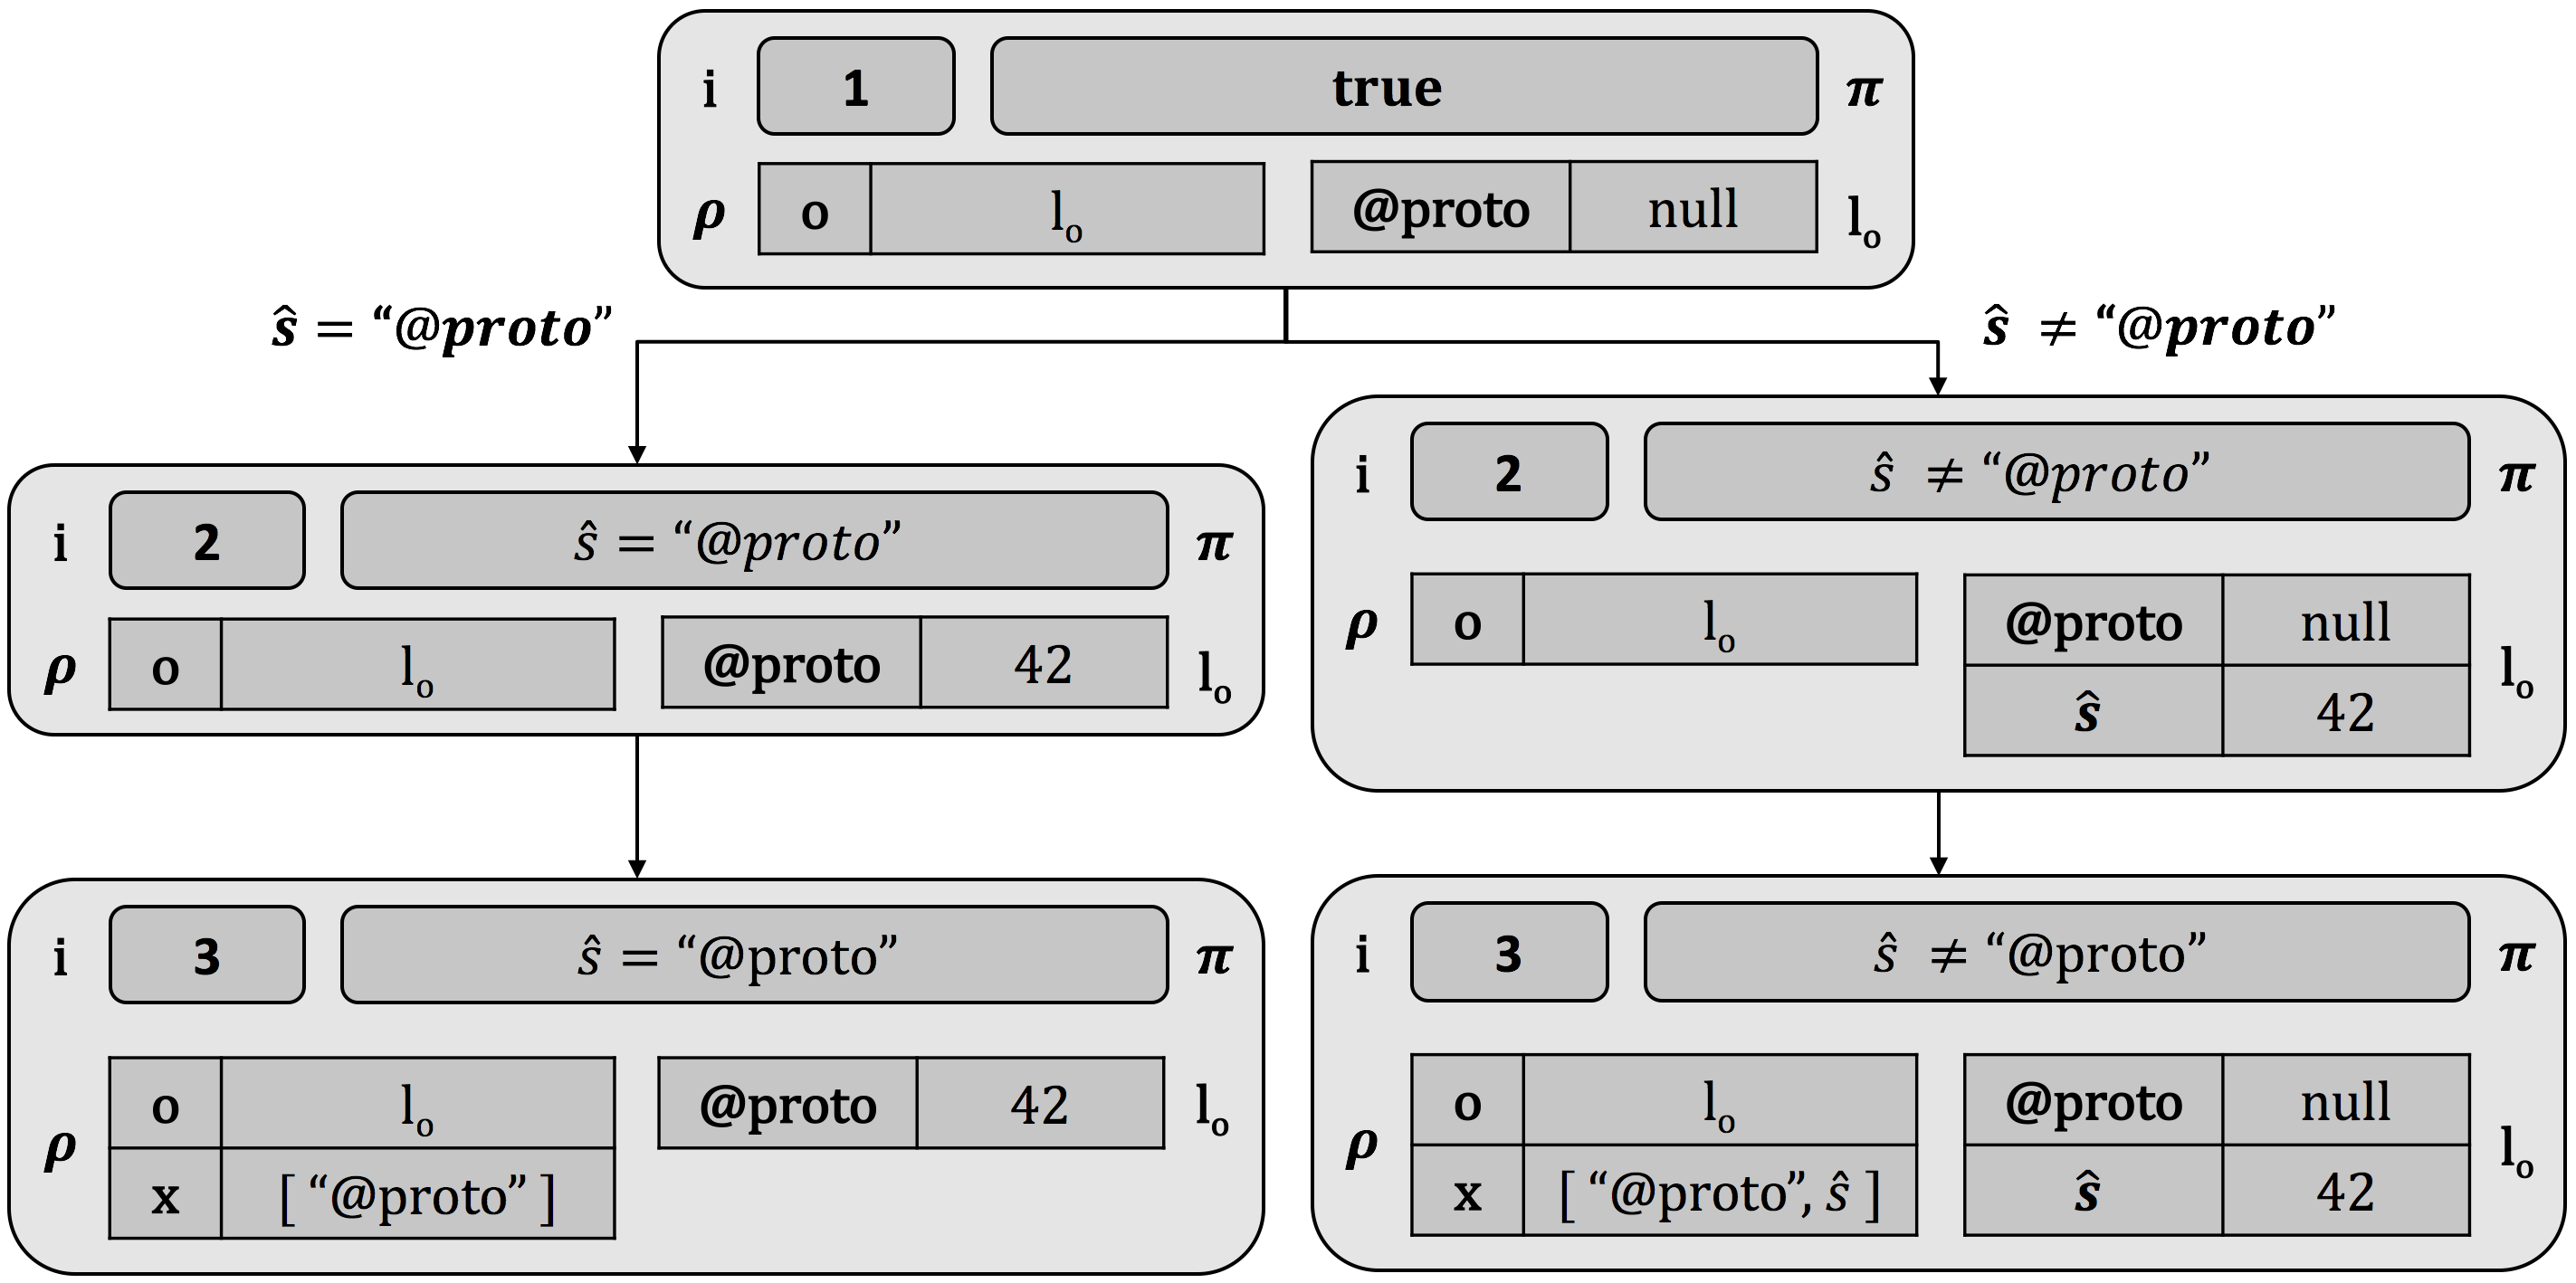
\includegraphics[width=0.83\textwidth]{symbSemEx.png}
\vspace*{-0.1cm}
\caption{Example of a \jilette symbolic execution}
\label{fig:sexecexample}
\vspace*{-0.3cm}
\end{figure}




%\caption{Concrete Semantics Rules}
%\end{figure}


% Given a heap~$\heap$, we denote: a heap cell by $\hcell{\loc}{\jstring}{\val}$, meaning that  $h(\loc,\jstring) = \val$; the union of two disjoint heaps by $\oheap_1 \dunion \oheap_2$; heap lookup by $\hread{\oheap}{\loc}{\jstring}$; and the empty heap by $\hemp$.
%A \jsil variable store, $\store \in \stores$, is a mapping from JSIL program variables $\jvar \in \jvars$ to JSIL values. 



%the heap $\heap'$, store $\store'$, call stack $\ctx'$,   
%and the next command to be evaluated is the $i'$-th command of the first procedure of the call stack~$\ctx'$, in execution mode $\mode'$

%the heap $\heap$, store $\store$, . Due to space constraints and as the transitions for JSIL symbolic execution are  similar, we give the full semantics for JSIL control flow commands in the~Appendix. % So far, so boring.




%We denote the semantic interpretation of unary operators $\unoper$ by $\semop{\unoper}$, the semantic interpretation of binary operators $\binoper$ by $\semop{\binoper}


\subsection{Formal Guarantees}\label{sex:formal:guarantees}

\subsection{Implementation}\label{subsec:jsil:analysis:implementation}

%
%\myparagraph{\jsil: Symbolic Semantics}
%
%Figure~\ref{fig:symbexe:cmds} presents the symbolic execution rules for \jsil commands. 
%Rules have the form $\symbtrans[\prog][\mode][\mode']{\sheap, \sstore, i, \pc}{\sheap', \sstore', i', \pc'}[\sctx][\sctx']$; 
%they are analogous to the semantic rules for \jsil commands, except that the heap, store, and call stack 
%are symbolic and there is the additional path condition. 
%
%\begin{wrapfigure}{R}{0.4\textwidth}
%\vspace*{-0.25cm}
%{\small
%\hspace*{0.25cm} $\mathtt{0\quad o := new\ ()}$ \\
%\hspace*{0.25cm} $\mathtt{1\quad o[\hat{s}] := 42};$ \\
%\hspace*{0.25cm} $\mathtt{2\quad x := getFields(o);}$ \\
%\hspace*{0.25cm} $\mathtt{3\quad assert\ (card \ x == 2)}$
%}
%\vspace*{-0.3cm}
%\end{wrapfigure}
%The rules for skip, assignment, object creation, property collection, assume, and assert are straightforward. The remaining rules follow a specific pattern. To get a better intuition of how these rules work, let us take a look at the snippet of code shown on the right. 
%This code: 
%	0)~creates a new object $\mathtt{o}$;
%	1)~assigns 42 to a symbolic property $\mathtt{\hat{s}}$ of $\mathtt{o}$; 
%	2)~collects all the properties of $\mathtt{o}$ into a set and assigns this set to $\mathtt{x}$; and
%	3)~asserts that the cardinality of the set in $\mathtt{x}$ is 2, i.e.~that~$\mathtt{o}$ has two properties in the end. This last assertion will produce a failing symbolic execution. Let us understand why.
%
%We start from an empty heap, empty store, and an empty path condition: $\tuple{\hemp, \emptyset, 0, \jtrue}^\top$. After the execution of the first command, $\mathtt{o := new\ ()}$, using the \textsc{Basic Command} and \textsc{Object Creation} rules, we get to the state {\small $\tuple{\{ \mathtt{l_o : \{ ``@proto" : null} \} \}, \{ \mathtt{o : l_o} \} , 1, \jtrue}^\top$}, illustrated at the top of Figure~\ref{fig:sexecexample}.
%The next command to be executed is the property assignment $\mathtt{o[\hat{s}] := 42}$. In the symbolic semantics, there are two potential \textsc{Property Assignment} rules (\textsc{Found}, \textsc{Not Found}), and in our case, both of them are applicable. The key strategy is to branch on the targeted property of the object (in our case, the symbolic property $\hat{s}$ of object at location $\mathtt{l_o}$) being equal to any one or none of the already existing properties of the object (in our case, we have only $\mathtt{``@proto"}$), adding the appropriate equalities and inequalities to the path condition, and proceeding with the symbolic execution for all obtained branches. In this case, this means that the symbolic execution will branch on whether or not $\hat{s} = \mathtt{``@proto"}$. We obtain two symbolic states, shown in the second row of Figure \ref{fig:sexecexample}. The left branch corresponds to the (\textsc{Found}) case, when $\hat{s} = \mathtt{``@proto"}$: this equality is added to the path condition and the value of the property $\mathtt{``@proto"}$ is updated to 42. In the right branch, we have that $\hat{s} \neq \mathtt{``@proto"}$ (\textsc{Not Found}), hence object $\mathtt{o}$ has two properties: $ \mathtt{``@proto"}$, with value $\jsnull$; and $\hat{s}$, with value 42.
%The execution then continues in both branches with the property collection command $\mathtt{x := getFields(o)}$, which assigns the set of properties of the object $\mathtt{o}$ to the variable~$\mathtt{x}$ (last row of Figure~\ref{fig:sexecexample}). Finally, we execute $\mathtt{assert\ (card \ x = 2)}$, asserting that $\mathtt{o}$ has exactly two properties, which we observe to hold in the right branch, but not in the left.
%Therefore, following the \textsc{Assert - False} rule, we obtain a failing symbolic execution trace, from which a concrete counter-model can be derived ($\hat{s} = \mathtt{``@proto"}$).
%
%We now present our theoretical results. We denote the reflexive-transitive closure of $\rightarrow$ by $\rightarrow^*$ and the reflexive-transitive closure of $\leadsto$ by $\leadsto^*$, and we define both in the usual way.
%
%%\vspace*{-0.3cm}
%\begin{figure}[!t]
%\centering
%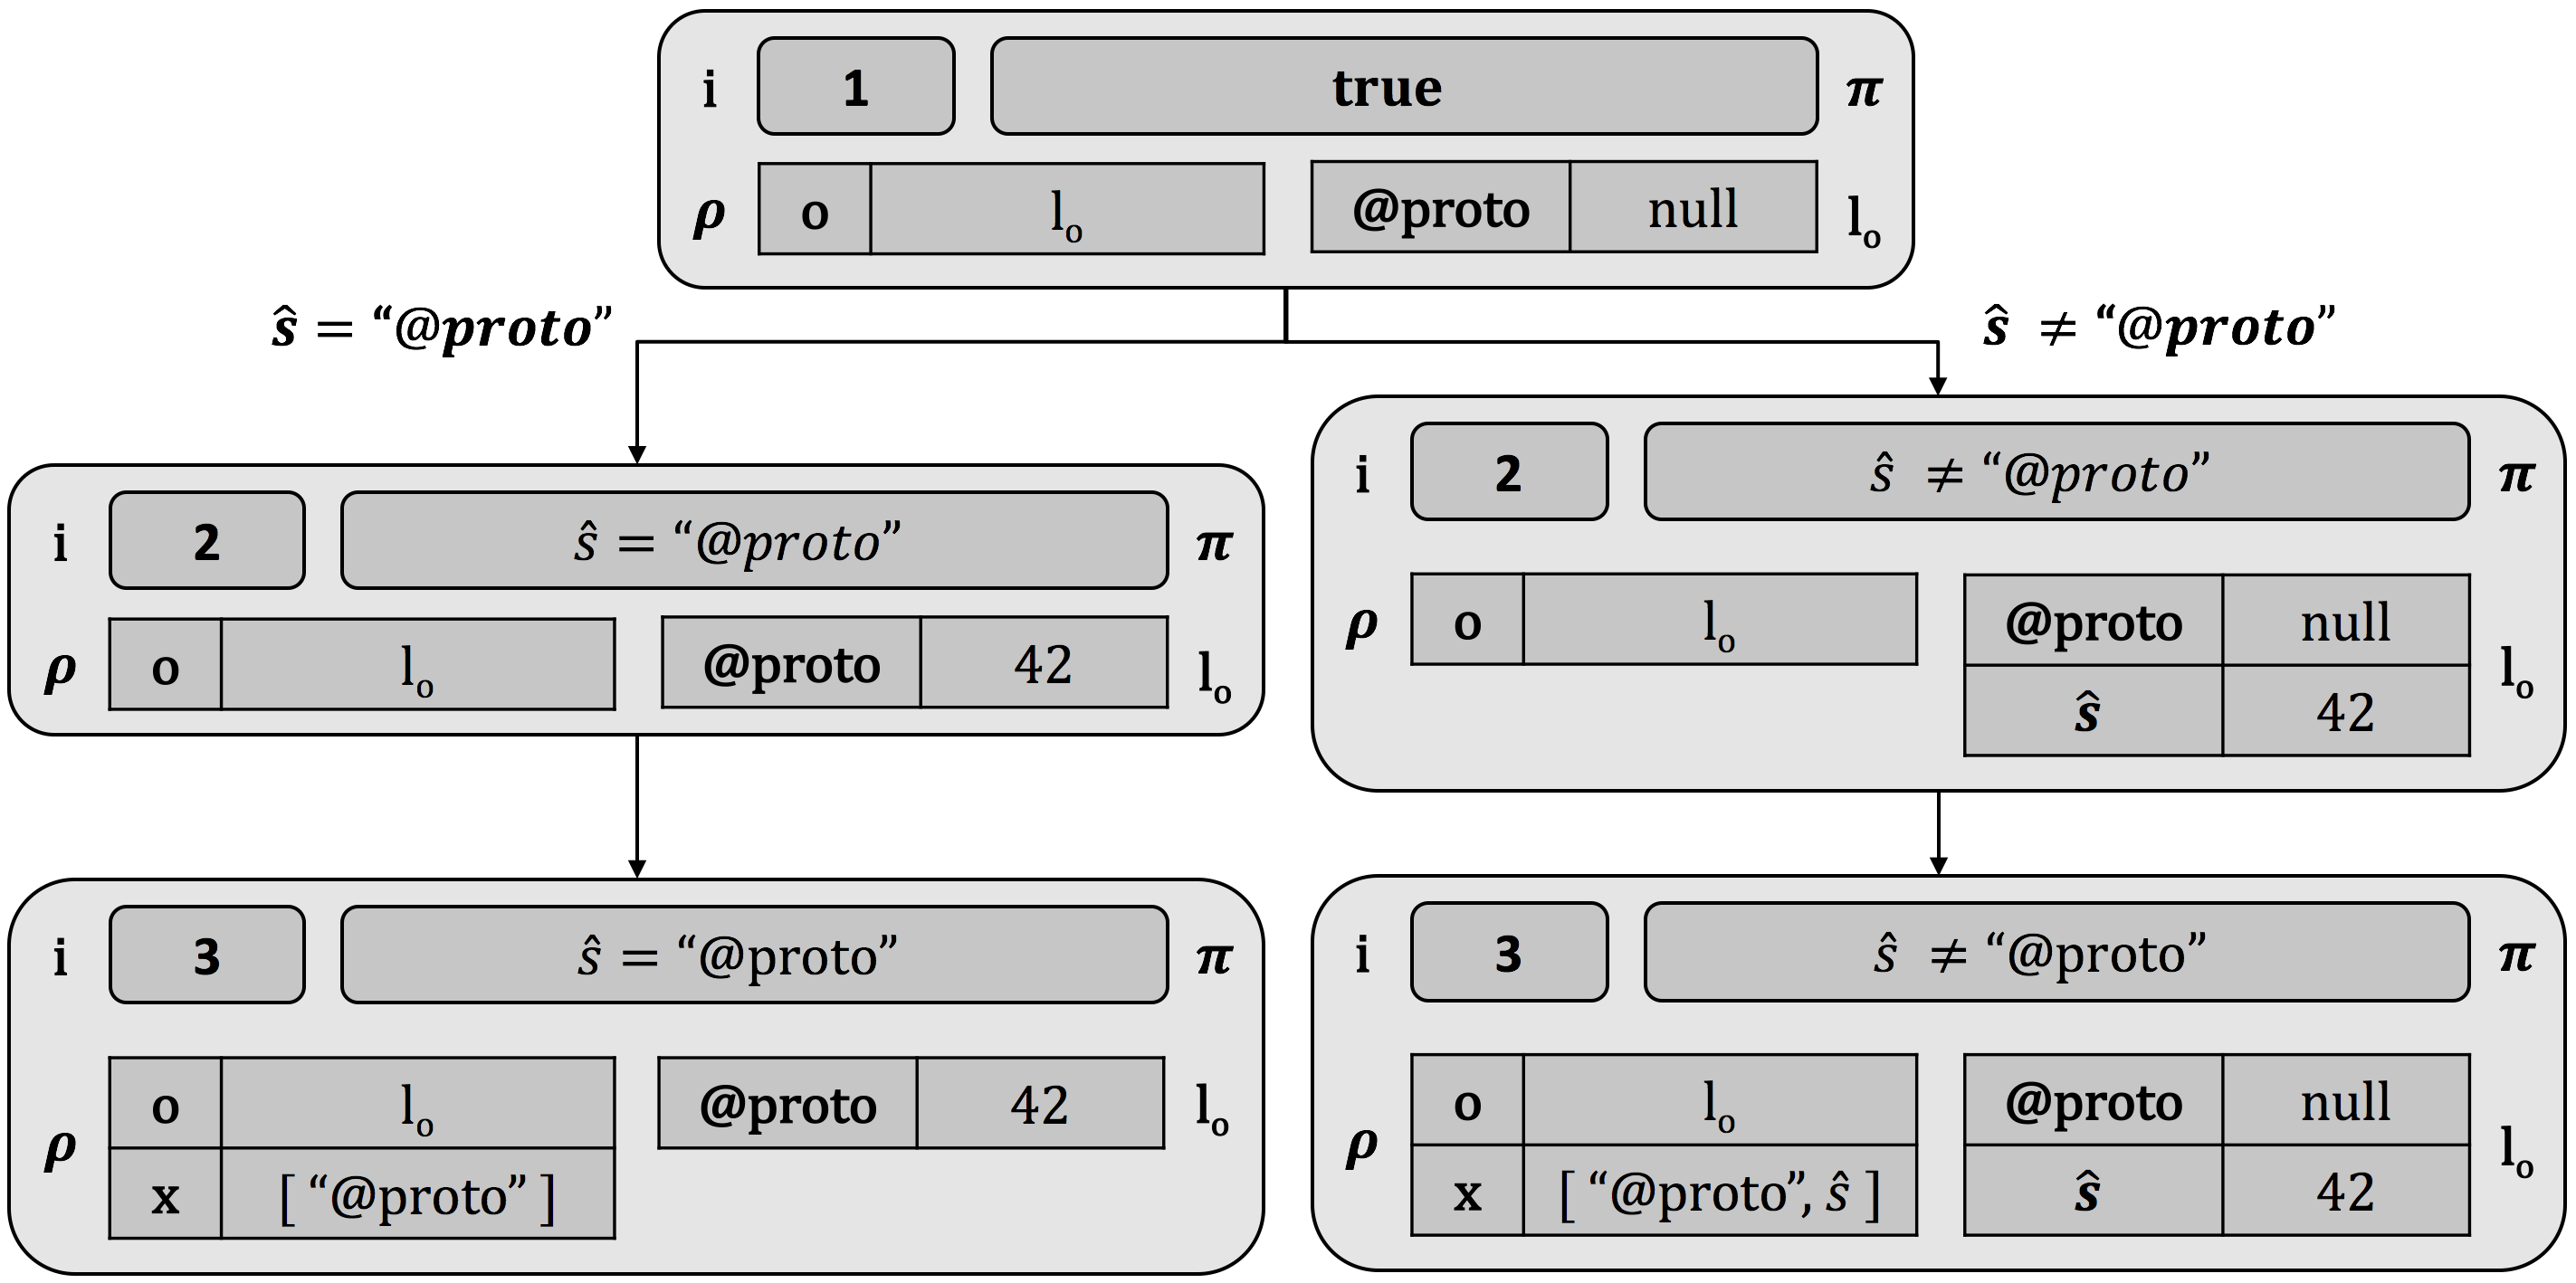
\includegraphics[width=0.83\textwidth]{symbSemEx.png}
%\vspace*{-0.1cm}
%\caption{Example of a \jilette symbolic execution}
%\label{fig:sexecexample}
%\vspace*{-0.3cm}
%\end{figure}
%
%\myparagraph{Transparency} 
%Observe that a concrete state is also a symbolic state. Hence, we can feed a concrete state to the 
%symbolic execution. In that case, the symbolic execution must behave exactly as the concrete 
%execution. This is captured by the transparency theorem given below. 
%
%\begin{theorem}[Transparency]\label{teo:transparency}
%$\forall \, \prog, \heap, \store, i, \ctx, \mode, \heap',  \store', i',  \ctx', \mode' \, . \,$
%\vspace{-5pt}
%$$
%  \semtranstrans[\prog][\mode][\mode']{\heap, \store, i}{\heap', \store', i'}[\ctx][\ctx']
%  \iff
%  \symbtranstrans[\prog][\mode][\mode']{\heap, \store, i, \jtrue}{\heap', \store', i', \jtrue}[\ctx][\ctx']. 
%$$
%\end{theorem}
%
%

%\myparagraph{Soundness} To establish the soundness of symbolic execution, we need to relate 
%symbolic states to concrete states. To this end, we make use of \emph{symbolic environments} 
%$\senv : \svars \rightharpoonup \vals$, mapping symbolic values to concrete values. 
%A symbolic environment is \emph{well-formed} if it maps symbolic 
%values to concrete values of the appropriate type (i.e.~symbolic strings are mapped to strings 
%and symbolic numbers are mapped to numbers). In the following, we always 
%assume well-formed symbolic environments. 
%%
%Given a symbolic environment $\senv$, we define the interpretation of extended expressions and symbolic expressions as follows:
%
%\begin{figure*}[!h]
%{\footnotesize
%\textsc{Interpretation of Symbolic Expressions}
%\vspace*{-0.1cm}
%\begin{mathpar}
%\semexpr{\val}{\senv} \semeq \val 
%%
%\qquad
%%
%\semexpr{\svar}{\senv} \semeq \senv(\svar)
%\qquad
%%
%\semexpr{\unoper\ \sexpr}{\senv} \semeq \semop{\unoper} (\semexpr{\sexpr}{\senv})
%\qquad 
%\semexpr{\sexpr_1 \binoper \sexpr_2}{\senv} \semeq \semop{\binoper}(\semexpr{\sexpr_1}{\senv}, \semexpr{\sexpr_2}{\senv}) 
%\end{mathpar}
%
%
%\textsc{Interpretation of Extended Expressions}
%\vspace*{-0.2cm}
%\begin{mathpar}
%{\begin{array}{c}
%\semexpr{\val}{\senv} \semeq \val \\[2pt]
%%
%\semexpr{\xvar}{\senv} \semeq \xvar \\[2pt]
%%
%\semexpr{\svar}{\senv} \semeq \senv(\svar)
%\end{array}}
%\quad
%%
%\frac{\semexpr{\pvsexpr}{\senv} = \val}
%      {\semexpr{\unoper\ \pvsexpr}{\senv} \semeq \semop{\unoper} \val}
%%
%\quad
%%
%\frac{\semexpr{\pvsexpr}{\senv} = \pvsexpr' \not\in \vals}
%       {\semexpr{\unoper\ \pvsexpr}{\senv} \semeq \unoper \ \pvsexpr'}
%%
%\quad
%\frac{ \val = \semop{\binoper}(\semexpr{\pvsexpr_1}{\senv}, \semexpr{\pvsexpr_2}{\sstore})} 
%       {\semexpr{\pvsexpr_1 \binoper \pvsexpr_2}{\senv} \semeq \val}
% %
% \quad
%\frac{{\begin{array}{c}
%	\semexpr{\pvsexpr_1}{\senv} = \pvsexpr_1' 
%	  \quad 
%	  \semexpr{\pvsexpr_2}{\senv} = \pvsexpr_2'
%	  \\
%	  \pvsexpr_1' \not\in \vals \ \vee \ \pvsexpr_2' \not\in \vals 
%	  \end{array}}
%	}
%	{\semexpr{\pvsexpr_1 \binoper \pvsexpr_2}{\senv} \semeq \pvsexpr_1' \, {\binoper} \, \pvsexpr_2'}
%\end{mathpar}}
%\vspace*{-0.4cm}
%\end{figure*}
%
%We extend this interpretation to heaps, stores, contexts, basic commands, commands, procedures, and programs in the standard way, shown in the Appendix.  
%We say that a symbolic environment is \emph{consistent} with a path condition 
%$\pc$, written $\senv \vdash \pc$,  if and only if $\semexpr{\pc}{\senv} = \jtrue$. 
%Given a symbolic state $(\sheap, \sstore, \sctx)$ and a path condition $\pc$, we define 
%the models of the symbolic state under $\pc$, written $\smodels{\sheap, \sstore, \sctx}{\pc}$, 
%as the set of concrete states that can be obtained from $(\sheap, \sstore, \sctx)$ using 
%symbolic environments that are consistent with~$\pc$. Formally:
%
%{\small \begin{align}
%\smodels{\sheap, \sstore, \sctx}{\pc} & = \left\{ (\heap, \store, \ctx, \senv) \mid \semexpr{(\sheap, \sstore, \sctx)}{\senv} = (\heap, \store, \ctx) \, \wedge \,  \senv \satisfies \pc  \right\} \\
%\smodels{\sheap, \sstore}{\pc} & = \left\{ (\heap, \store, \senv) \mid \semexpr{\sheap}{\senv} = \heap \, \wedge \, \semexpr{\sstore}{\senv} = \store \, \wedge \,  \senv \satisfies \pc  \right\}
%\end{align}}
%
%%\begin{figure}[t!]
%%{\small
%%\begin{tabular}{l}
%%$\quad${\bf Interpretation of Symbolic Expressions:}  \\
%%$
%%\quad
%%\semexpr{\val}{\senv} \semeq \val
%%\quad 
%%\semexpr{\jvar}{\senv} \semeq \jvar
%%\quad 
%%\semexpr{\svar}{\senv} \semeq \senv(\svar)
%%\quad 
%%\semexpr{\unoper\ \sexpr}{\senv} \semeq \semop{\unoper} (\semexpr{\sexpr}{\senv})
%%\quad 
%%\semexpr{\sexpr_1 \binoper \sexpr_2}{\senv} \semeq \semop{\binoper}(\semexpr{\sexpr_1}{\senv}, \semexpr{\sexpr_2}{\senv}) 
%%$
%%\\[3pt]
%%$\quad${\bf Symbolic Heaps:}  \\
%%$
%%\quad
%% \semexpr{\hemp}{\senv} \semeq \hemp
%%\quad
%%\semexpr{\hcell{\loc}{\sexpr_p}{\sexpr_v}}{\senv} \semeq  \hcell{\loc}{\semexpr{\sexpr_p}{\senv}}{\semexpr{\sexpr_v}{\senv}}
%%\quad
%%\semexpr{\sheap_1 \dunion \sheap_2}{\senv} \semeq  \semexpr{\sheap_1}{\senv} \dunion \semexpr{\sheap_2}{\senv}
%%$%
%%%%
%%%%
%%\\[3pt]
%%$\quad${\bf Symbolic Stores:}  
%%$
%% \semexpr{\storeemp}{\senv} \semeq \storeemp
%%\quad 
%% \semexpr{(\jvar: \sexpr) \dunion \sstore}{\senv} \semeq (\jvar: \semexpr{\sexpr}{\senv}) \dunion \semexpr{\sstore}{\senv}
%%$%
%%\\[3pt]
%%$\quad${\bf Symbolic Contexts:}  
%%$ \semexpr{\lstemp}{\senv} \semeq \lstemp
%%\quad 
%% \semexpr{(\pid, \sstore, \jvar, i, j) \lstcons \sctx}{\senv} \semeq (\pid, \semexpr{\sstore}{\senv}, \jvar, i, j) \lstcons \semexpr{\sctx}{\senv}
%%$%
%%
%%\\[3pt]
%%$\quad${\bf Symbolic States:}  $\semexpr{(\sheap, \sstore, \sctx)}{\senv} \semeq (\semexpr{\sheap}{\senv}, \semexpr{\sstore}{\senv}, \semexpr{\sctx}{\senv})$
%%\end{tabular}
%%}
%%\caption{Interpretation of symbolic expressions, heaps, stores, and contexts.\label{fig:symbolic:interp}}
%%\vspace{-0.5cm}
%%\end{figure}
%
%\vspace*{-0.3cm}
%The soundness theorem (Theorem~\ref{teo:soundness:jsil:symb:exe}) states that if we have a symbolic trace captured by 
%$\symbtranstrans[\prog][\mode][\mode']{\sheap, \sstore, i, \pc}{\sheap', \sstore', i', \pc'}[\sctx][\sctx']$ 
%and a concrete state $(\heap, \store, \ctx)$ with a symbolic environment~$\senv$
%in the models of the initial symbolic state under 
%the final path condition $\pc'$, and $\senv$ concretises all symbolic variables of the program $\prog$, then there exists a concrete symbolic state $(\heap', \store', \ctx')$ 
%that is in the models of the final symbolic state under $\pc'$ with the same symbolic environment~$\senv$, such that: 
%$\semtranstrans[\symbeval{\prog}{\senv}][\mode][\mode']{\heap, \store, i}{\heap', \store', i'}[\ctx][\ctx']$. 
% We use the final path condition $\pc'$ for both the models of the initial and final 
%symbolic states because we only care about the initial concrete states for which 
%the concrete execution will follow the same path as the symbolic execution. 
%%
%\begin{theorem}[Soundness]\label{teo:soundness:jsil:symb:exe}
%$\forall \, \prog, 
%	\sheap, \sstore, i, \pc, \sctx, \mode, 
%	\sheap', \sstore', i', \pc', \sctx', \mode', 
%	\heap, \store, \ctx, \senv \, .$
%\vspace*{-0.65cm}
%$$
%\begin{array}{l}
%\\  
%\quad \symbtranstrans[\prog][\mode][\mode']{\sheap, \sstore, i, \pc}{\sheap', \sstore', i', \pc'}[\sctx][\sctx'] 
%   \ \wedge \ 
%      (\heap, \store, \ctx, \senv) \in \smodels{\sheap, \sstore, \sctx}{\pc'} \\ \quad \quad
%      	 \ \Rightarrow \ \exists \heap', \store', \ctx' \, . \, 
%	 	 \semtranstrans[\symbeval{\prog}{\senv}][\mode][\mode']{\heap, \store, i}{\heap', \store', i'}[\ctx][\ctx']
%		\, \wedge \, 
%		(\heap', \store', \ctx') \in \smodels{\sheap', \sstore', \sctx'}{\pc'}  
%\end{array}
%$$
%\end{theorem}
%%
%The \emph{bug-finding} corollary (Corollary~\ref{bug:finding}) states that if 
%we find a symbolic trace that results in a failed assertion, 
%then there also exists a concrete execution that will cause that assertion to fail.
%Observe that the analysis is designed in such a way that there are no false positives, 
%meaning that if we find a failing symbolic trace,
%we can always instantiate its symbolic values obtaining a concrete counter-model for the 
%failing assertion. This is essential, as \jilette is meant to be a \emph{bug-finding} tool.
%%
%\begin{corollary}[Bug-finding]\label{bug:finding}
%$\forall \, \prog, \sheap, \sstore, i, \pc, \sctx, \sheap', \sstore', j, \pc', \sctx' \, .$
%\vspace*{-0.2cm}
%$$
%\begin{array}{l} 
% \quad \symbtranstrans[\prog][\top][\bot]{\sheap, \sstore, i, \pc}{\sheap', \sstore', j, \pc'}[\sctx][\sctx']  \\ 
%   \qquad \Rightarrow 
%     \exists \heap, \store, \ctx, \senv \, . \, (\heap, \store, \ctx, \senv) \in \smodels{\sheap, \sstore, \sctx}{\pc'} \ \wedge \ \semtranstrans[\symbeval{\prog}{\senv}][\top][\bot]{\heap, \store, i}{\_, \_, \_}[\ctx][\_]. 
%\end{array}
%$$
%\end{corollary}
%%
%Finally, the \emph{verification} corollary (Corollary~\ref{corollary:verification})
%states that if we have symbolically explored all the possible execution paths
%starting from a given symbolic state $(\sheap, \sstore, \sctx)$,  
%then the execution of the program starting from  any concrete state in the models 
%of the initial symbolic state (under the initial path condition) will result in a final concrete state
%in the models of one of the final symbolic states (under its associated path condition).  
%As \jilette does not infer loop invariants, if a \jsil program contains loops that cannot be unrolled statically, we will never be in the case of the verification corollary. 
%
%\begin{corollary}[Verification]\label{corollary:verification}
%$$
%\begin{array}{l}
%\forall \, \prog, \sheap, \sheap_1, ..., \sheap_n, \sstore, \sstore_1, ..., \sstore_n, \sctx, \sctx_1, ..., \sctx_n, i, j_1, ..., j_n, \pc, \pc_1, ..., \pc_n,\mode, \mode_1, ..., \mode_n. \\
%   \;\; \wedge_{k=1}^n \left(\symbtranstrans[\prog][\mode][\mode_k]{\sheap, \sstore, i, \pc}{\sheap_k, \sstore_k, j_k, \pc_k}[\sctx][\sctx_k]\mid_{k = 1}^n\right) 
%      \ \wedge \ \pc \vdash \bigvee_{k=1}^n \pc_k \\ 
%       \;\;\;\; \Rightarrow \left(
%         \forall \heap, \store, \ctx, \senv \, . \, (\heap, \store, \ctx, \senv) \in \smodels{\sheap, \sstore, \sctx}{\pc} \right. \\
%           \;\;\;\;\;\; \left. \Rightarrow \exists k, \heap', \store', \ctx' \, . \, 
%                  \semtranstrans[\symbeval{\prog}{\senv}][\mode][\mode_k]{\heap, \store, i}{\heap', \store', j_k}[\ctx][\ctx'] \ \wedge \ 
%                  (\heap', \store', \ctx', \senv) \in \smodels{\sheap_k, \sstore_k, \sctx_k}{\pc_k} \right)
%\end{array}
%$$ 
%\end{corollary}
%%
%The {\bf proofs} of the above results are given in the Appendix. \polish{What do these results mean with respect to related work? How is this maintainable?} 
%
%

%
%Implementing a symbolic execution engine for \jsil is a non-trivial 
%task, requiring a substantial engineering effort. 
%% 
%% 
%Hence, instead of implementing the symbolic semantics of \jsil from scratch, we leverage on 
%\rosette~\cite{Rosette1,Rosette2}, a symbolic virtual machine designed to 
%enable swift development of new 
%solver-aided languages. 
%%
%\rosette is a small extension of Racket~\cite{racket} equipped with a symbolic compiler with support 
%for symbolic values and first order assertions. Because \rosette is itself solver-aided, languages 
%implemented in \rosette can also make use of the solver-aided facilities provided by \rosette. 
%Hence, by implementing a \emph{concrete} \jsil interpreter in \rosette, we obtain \emph{for free} a symbolic 
%interpreter for \jsil. %consistent with the symbolic semantics described in  \S\ref{subsec:jsil:analysis:formalism}. 
%%The idea of turning a concrete interpreter into a symbolic interpreter by embedding it in 
%%
%The implementation of the concrete interpreter in \rosette must fulfil the following criteria:
%
%\begin{itemize}          
%   \item \emph{Efficiency:} the implementation must promote \rosette's efficient behaviour;
%   
%   \item \emph{Termination:} the user must be given a way to establish a bound for the symbolic execution 
%            of programs that loop on symbolic values; 
%  
%   \item \emph{Adequacy:} the symbolic execution of the concrete interpreter in \rosette 
%            must be consistent with the symbolic semantics described in \S\ref{subsec:jsil:analysis:formalism}. 
%            We discuss adequacy in \S\ref{sec:evaluation} in the context of the global evaluation 
%            of \jilette.
%\end{itemize}
%
%%- describe the \rosette approach to the implementation of symbolic analysis 
%% - describe the encoding of \jsil concrete/symbolic states in \rosette 
%% - explain the \jsil interpreter implemented in \rosette and its connection to the \jsil concrete semantics  and symbolic semantics 
%%- give snippets of the interpreter 
%%- discuss implementation strategies that enable \rosette to work properly
%
%\myparagraph{Implementing \jsil in \rosette}
%We first show
%how to model the concrete \jsil state. Below are our \rosette encodings of \jsil heaps, stores, 
%and call stacks. 
%Heaps are modelled as pairs of locations and lists of property-value pairs, 
%stores as lists of variable-value pairs, and call stacks as lists of lists, each of which
%contains the \rosette encoding of the appropriate four elements. 
%\jsil variables and function identifiers are modelled 
%as Racket symbols.\footnote{Racket symbols are uninterpreted values and can be viewed as immutable strings.} 
%\jsil values with \rosette correspondents are mapped accordingly; the remaining 
%ones are modelled as Racket symbols (e.g. \jsil types, $\jsundefined$, $\jsnull$, and $\jsilempty$). 
%
%The implementation of \jsil commands precisely follows their concrete semantics as 
%described in \S\ref{subsec:jsil:analysis:formalism}. 
%To show this, let us consider the fragment of the \jsil interpreter that implements 
%the \prooflab{Property Assignment} rule, shown in Figure~\ref{rosette:interpreter:fragment}.
%The figure shows three functions: \dtag{1} \schemeinline|(run-bcmd bcmd heap store)|, for 
%executing basic commands, \dtag{2} \schemeinline|(update-heap heap loc prop val)|, for 
%updating the heap \schemeinline|heap| by setting the value of the 
%the property \schemeinline|prop| of the object denoted by \schemeinline|loc| to \schemeinline|val|, 
%and \dtag{3} \schemeinline|(update-pv-list pv-list prop new-val)|,
%for updating the property-value list \schemeinline|pv-list| by setting \schemeinline|prop|
%to \schemeinline|new-val|.
%
%\begin{display}{\rosette implementation of the \jsil symbolic state}
%{\scriptsize
%\begin{mathpar}
%\inferrule[\textsc{Empty Heap}]
%  {}{\roscomp{\hemp} \semeq (\racketlist)} 
%\and 
%\inferrule[\textsc{Non-empty Heap}]
%  {
%  	 \sheap_1 = \big((l, \sexprp_i) \mapsto \sexprv_i\big)\mid_{i = 0}^n   
%	 \quad 
%	 (\loc, -) \not\in \domain(\sheap_2)
%  }{\roscomp{\sheap_1 \dunion \sheap_2} \semeq  (\racketcons (\racketcons \loc \, (\racketlist \, (\racketcons \sexprp_0 \, \sexprv_0) \cdots   (\racketcons \sexprp_n \, \sexprv_n)))  \ \roscomp{\sheap_2})} 
% \\
%\inferrule[\textsc{Empty Store}]
%  {}{\roscomp{\storeemp} \semeq (\racketlist)} 
%\and 
%\inferrule[\textsc{Non-Empty Store}]
%  {}{\roscomp{(\jvar: \sexpr) \dunion \sstore} \semeq (\racketcons \, (\racketcons \, (\racketquote \jvar) \ \sexpr) \,  \roscomp{\sstore})} 
%\\ 
%\inferrule[\textsc{Empty Context}]
%  {}{\roscomp{\lstemp} \semeq (\racketlist)} 
%\quad 
%\inferrule[\textsc{Non-Empty Context}]
%  {}{\roscomp{(\fid, \sstore, \jvar, i, j) \lstcons \sctx} \semeq  (\racketcons \,  (\racketlist \, (\racketquote \fid) \, \roscomp{\sstore} \, (\racketquote \jvar) \, i \, j) \, \roscomp{\sctx})} 
%\end{mathpar}}
%\end{display}
%
% 
%
%\lstset{language=Scheme, numbers = left}
%
%\begin{figure}[t!]
%\centering
%\begin{lstlisting}
%(define (run-bcmd bcmd heap store)
%  (let ((cmd-type (first bcmd)))
%    (cond
%    	[(eq? cmd-type 'p-assign)
%      	 (let* ((loc-val  (run-expr (second bcmd) store))
%                (prop-val (run-expr (third bcmd)  store))
%                (rhs-val  (run-expr (fourth bcmd) store)))
%            (cons (update-heap heap loc-val prop-val rhs-val) store))]
%         ...)))
%\end{lstlisting}
%
%\begin{lstlisting}
%(define (update-heap heap loc prop val)
%  (cond
%    [(null? heap) (error "Inexistent object")]
%    [(equal? (caar heap) loc)
%       (cons (cons loc (update-pv-list (cdar heap) prop val)) (cdr heap))]
%    [ else (cons (car heap) (update-heap (cdr heap) loc prop val))]))
%\end{lstlisting}
%
%\begin{lstlisting}         
%(define (update-pv-list pv-list prop new-val)
%  (cond
%    [(null? pv-list) (list (cons prop new-val))]
%    [(equal? (caar pv-list) prop) (cons (cons prop new-val) (cdr pv-list))]
%    [ else (cons (car pv-list) (update-pv-list (cdr pv-list) prop new-val))]))
%\end{lstlisting}
%\vspace*{-0.3cm}
%\caption{Fragment of the \jsil Interpreter in \rosette\label{rosette:interpreter:fragment}}
%\vspace*{-0.5cm}
%\end{figure}
%
%\jsil commands are represented in \rosette as \emph{s-expressions}. 
% For instance, the property assignment basic command $[\jsilexpr_1, \jsilexpr_2] := \jsilexpr_3$
% is represented as: 
%
%\vspace*{-0.2cm}
%{\small $$
%\mathtt{(list \ (quote\ {p\text{--}assign}) \ \roscomp{\jsilexpr_1} \ \roscomp{\jsilexpr_2} \ \roscomp{\jsilexpr_3})}
%$$}
%\vspace*{-0.4cm}
%
%\noindent Therefore, the interpreter of basic commands first checks if the first element of the 
%list representing the command is equal to \schemeinline|p-assign|. If it is, 
%it uses the function \schemeinline|run-expr| to evaluate the three \jsil expressions 
%comprising the property-assignment in the appropriate order. Then, it invokes the 
%function \schemeinline|update-heap| to perform the actual update. 
%The function \schemeinline|update-heap| recursively iterates over all heap objects
%to find the object whose property is to be updated and, when it finds it, 
%uses the function \schemeinline|update-pv-list| to update the corresponding 
%field-value list. If it does not find it, it will raise an error. However, due to the concrete semantics of \jsil, this case is never triggered.
%
%\lstset{language=Scheme, numbers=none, backgroundcolor=\color{mygray}}
%\myparagraph{Efficiency}
%It is often possible for more than one transition of the symbolic 
%semantics to be applicable during symbolic execution, 
%giving rise to a potentially intractable number of possible symbolic states. 
%To counter this problem, \rosette uses a sophisticated 
%symbolic state merging algorithm, which factors out the common 
%part between multiple symbolic states  in order to expose more 
%opportunities for concrete evaluation. The non-mergeable portions of the state 
%are represented as \emph{guarded symbolic unions}. 
%Our goal is to write the interpreter code in a way that helps 
%\rosette merge sets of possible symbolic states, yielding minimal 
%guarded symbolic unions.
%To illustrate this point, let us consider the symbolic execution 
%of the property assignment $\mathtt{o[\hat{s}] := 42}$ in the 
%symbolic heap represented in \rosette as follows: 
%%
%%\smallskip
%%\noindent
%%\begin{BVerbatim}[fontsize=\footnotesize,commandchars=\$\{\},bgcolor=Gainsboro]
%%(lo (("@proto" null) ("a" 0) ("b" 1))) $phantom{xxxxxxxxxxxxxxxxxxxxxxxxxxxxxxxxxxxxxxxxxxxxxxxxx}
%%\end{BVerbatim}
%%
%%\smallskip
%%\noindent
%%with a symbolic store mapping \schemeinline|o| to \schemeinline|lo| and 
%%the path condition {\small $\mathtt{\hat{s} = \text{\texttt{"a"}} \ \vee \hat{s} = \text{\texttt{"b"}}}$}.
%%The two resulting symbolic heaps are represented in \rosette as:  
%%
%%\smallskip
%%\noindent
%%\begin{BVerbatim}[fontsize=\footnotesize,commandchars=\$\{\},bgcolor=Gainsboro]
%%(lo (("@proto" null) ("a" (? (= $shat "a") 42 0)) ("b" (? (= $shat "b") 42 1))) $phantom{xxxxxxxxxxxxxxxx}
%%\end{BVerbatim}
%%
%\smallskip
%\noindent
%Here, \rosette manages to push the guarded unions to 
%the object cells that may be affected by the property assignment, maintaining a common 
%property-value list for both resulting symbolic states. 
%Now, let us change the code of line 6 of \schemeinline|update-pv-list| 
%(in Figure~\ref{rosette:interpreter:fragment}) to:  
%
%%\smallskip
%%\noindent
%%\begin{BVerbatim}[fontsize=\footnotesize,commandchars=\$\{\},bgcolor=Gainsboro]
%%(append (cdr pv-list) (cons prop new-val)) $phantom{xxxxxxxxxxxxxxxxxxxxxxxxxxxxxxxxxxxxxxxxxxxxx}
%%\end{BVerbatim}
%
%\smallskip
%\noindent
%This change in the interpreter makes the order of the cells in the property-value 
%list change depending on which property gets updated. 
%Now, \rosette needs to create a single guarded union 
%with the two possible resulting property-value lists: 
%
%%\smallskip
%%\noindent
%%\begin{BVerbatim}[fontsize=\footnotesize,commandchars=\$\{\},bgcolor=Gainsboro]
%%(lo (? (= $shat "a") (("@proto" null) ("b" 1) ("a" 42)) (("@proto" null) ("a" 0) ("b" 42)))) 
%%\end{BVerbatim}
%
%\myparagraph{Termination} The \jsil symbolic execution engine does not 
%include the abstraction mechanisms which would allow it to finitise the symbolic 
%execution of loops depending on symbolic values~\cite{abstract:symbolic:exec}. 
%Hence, the user is asked to specify an upper bound on the number of times
%the symbolic execution is allowed to branch on symbolic values by using
%conditional gotos. 
%Once that upper bound is reached, if a conditional goto that branches 
%on a symbolic value is encountered, the symbolic execution stops.  
%
%%
%%\myparagraph{Adequacy} 
%%We strongly believe that the symbolic execution of the concrete interpreter 
%%in \rosette is consistent with respect to the \jsil symbolic semantics. 
%%In fact, we have ``reverse-engineered'' our \jsil symbolic execution by 
%%observing in detail the guarded unions produced by Rosette for each of 
%%the \jsil commands. Due to its complexity and scale, 
%%{a formal proof would require
%%mechanisation}, which is, unfortunately, beyond our manpower.
% 
%%Hence, the user is asked to specify an upper bound on the number of times
%%the symbolic execution is allowed to branch depending on symbolic values. 
%%Once that upper bound is reached, if a conditional goto that branches 
%%on a symbolic value is encountered, the symbolic execution simply stops.  
%
%\lstset{backgroundcolor=\color{white}}
%
%\section{Symbolic Testing for JavaScript}
%\label{sec:sym:exec:js}
%
%\begin{wrapfigure}{R}{0.58\textwidth}
%\vspace*{-0.4cm}
%\centering
%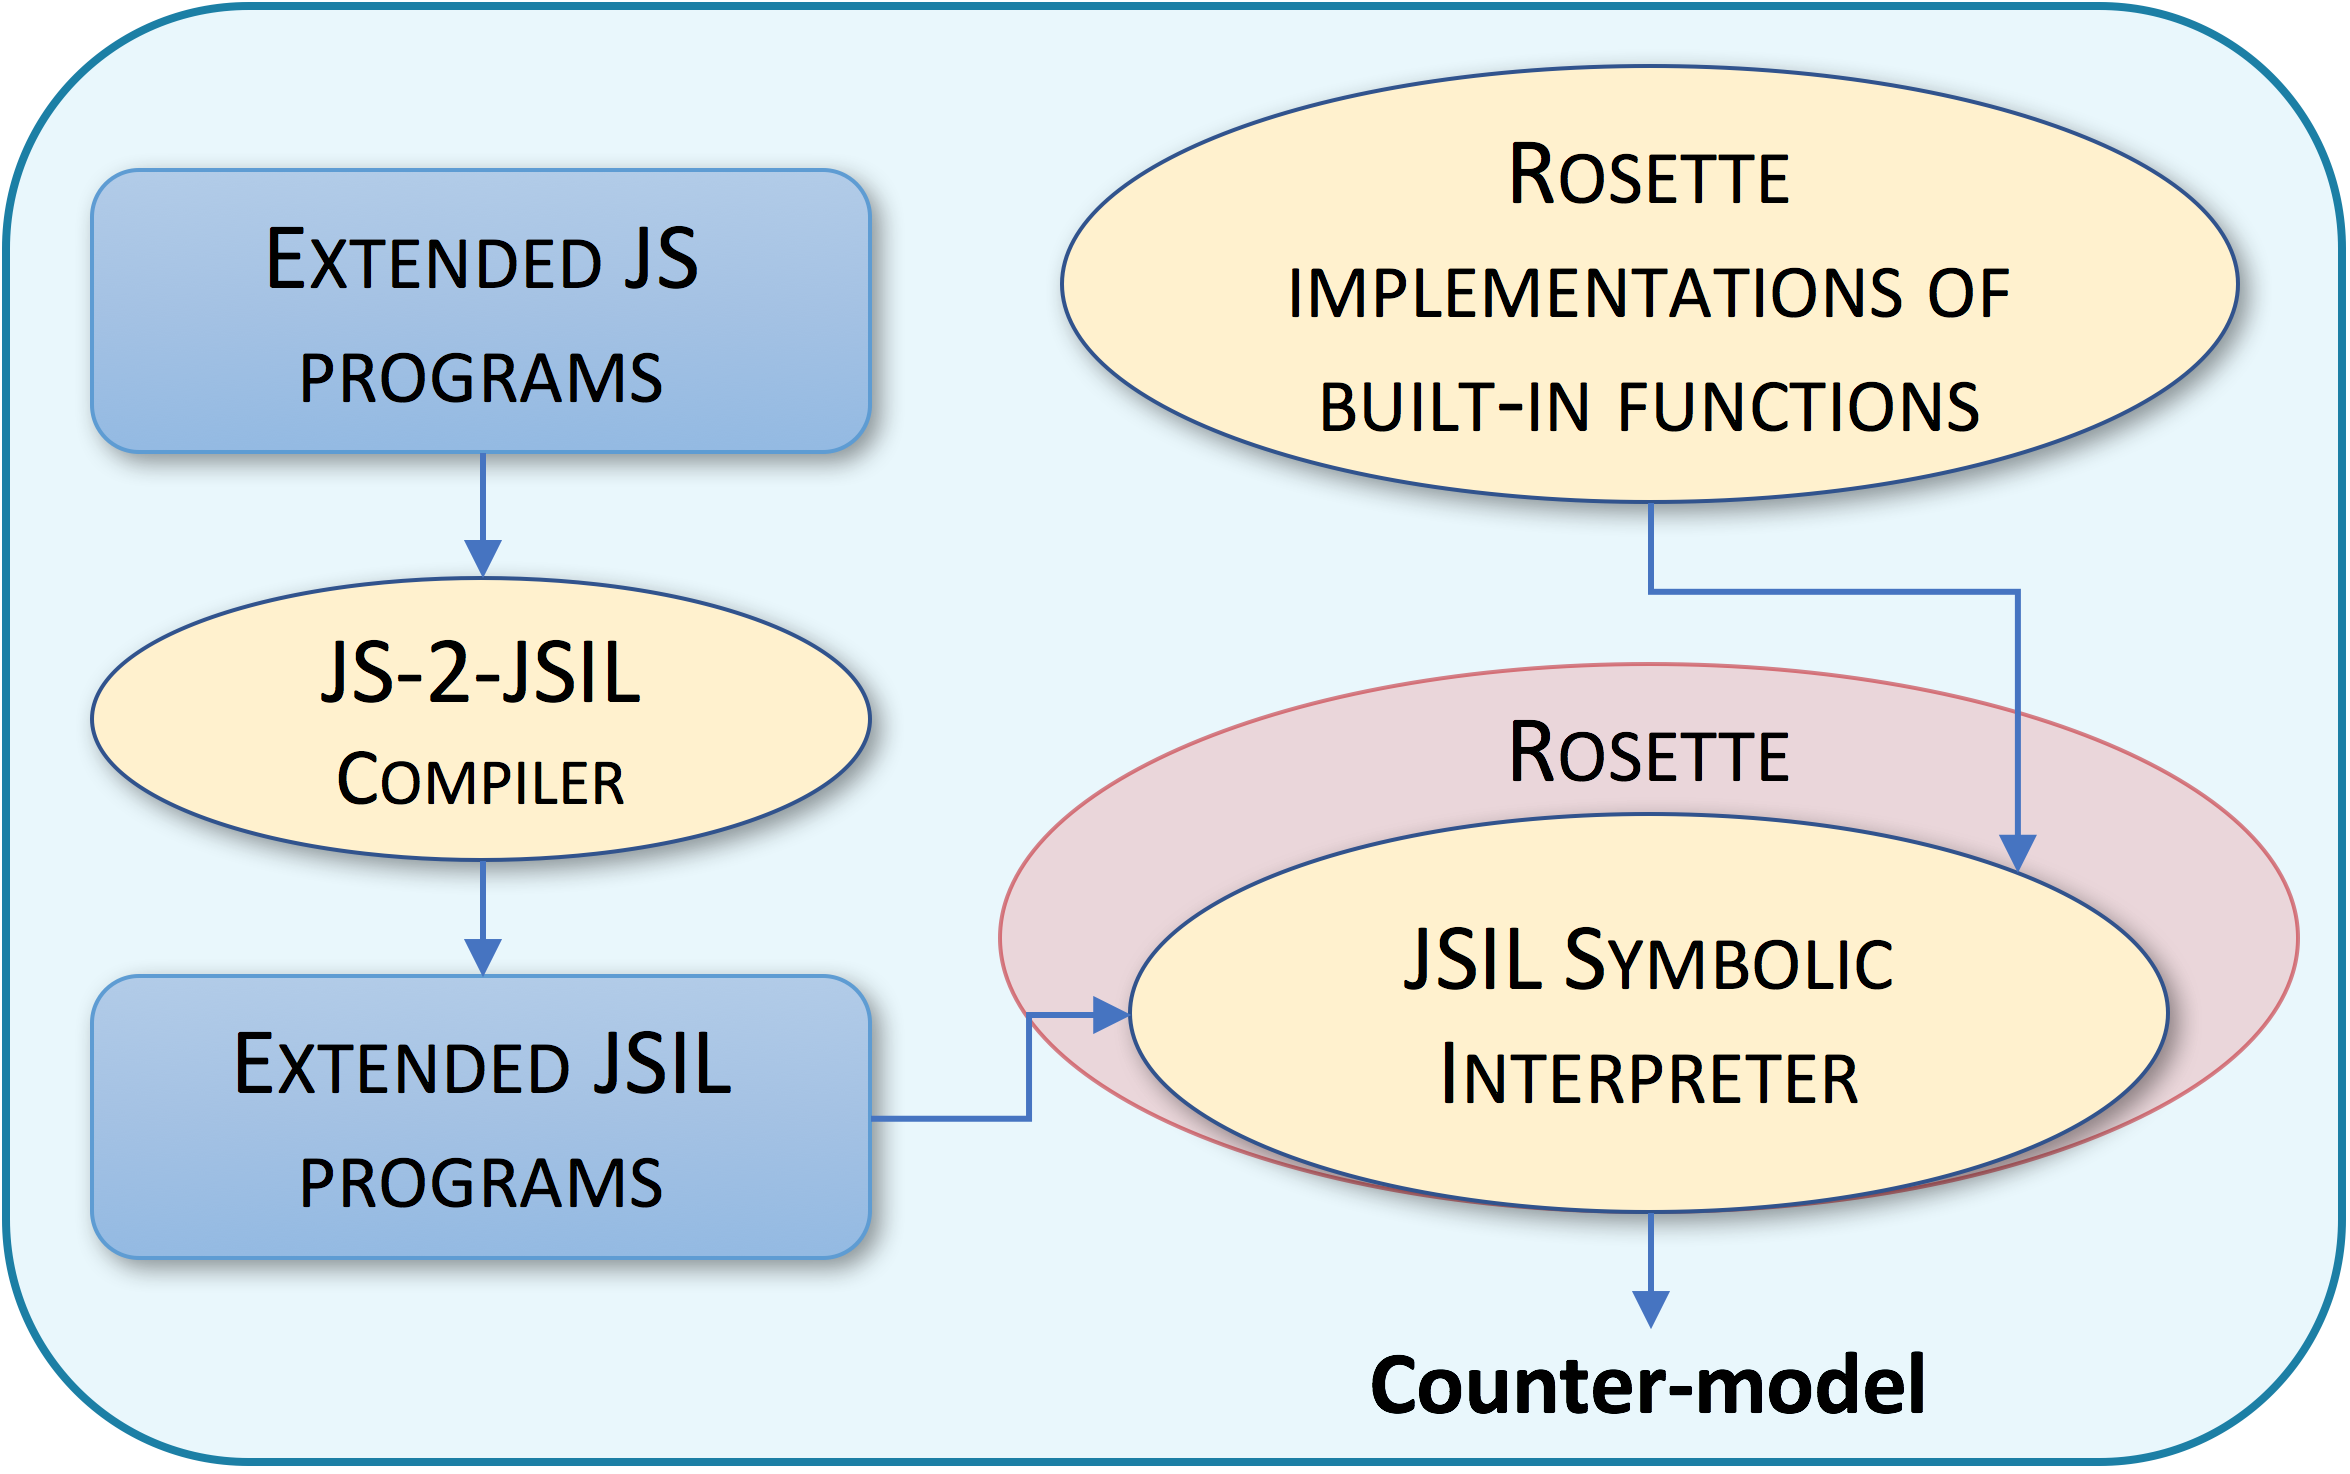
\includegraphics[width=0.57\textwidth]{figures/jilette_blue.png}
%\vspace*{-0.2cm}
%\caption{\jilette: Symbolic execution for JavaScript}
%\vspace*{-0.3cm}
%\label{fig:jilette:diagram}
%\end{wrapfigure}
%
%Symbolic execution designed directly on JavaScript is not feasible, for the same reasons verification is not~\cite{JoseCADE}: the semantics of the language is too complex, with numerous intertwined internal functions called under the hood. 
%In particular, the simple assignment alone would have more than twenty potential branchings. 
%Our approach is to symbolically analyse JavaScript code by first compiling it to \jsil, using~\JSComp~\cite{javert}, and then feeding the compiled \jsil code to our \jsil symbolic interpreter, described in \S\ref{sec:jsil:symb:exec}.
%
%In \S\ref{symb:exec:comp}, we explain how we enable symbolic execution for JavaScript using \JSComp and Rosette, by extending the language with new constructs for the creation of symbolic values and the checking of assertions.
%Next, in \S\ref{symbolic:testing}, we explain how this symbolic execution can be used for systematic symbolic testing of JavaScript code. 
%Finally, in \S\ref{builtins}, we present
%a general approach for streamlined symbolic execution of JavaScript built-in libraries, which maximises the use of Rosette's native solver-aided facilities.
%
%%More concretely, we extend the \jsil symbolic interpreter with \rosette implementations of JavaScript built-in libraries in a streamlined manner.  
%%These implementations are both an easy way to get a better coverage of the standard and 
%%match the abstraction level of the generated JSIL code precisely with the abstraction level 
%%of Rosette, maximising the use of Rosette's native solver-aided facilities.
%
%%to make sure that we make proper use of theof \rosette.    
%
%\subsection{Symbolic Execution by Compilation} 
%\label{symb:exec:comp}
%
%\myparagraph{Extending JavaScript Syntax}
%We extend the syntax of JavaScript with logical expressions $\jslexpr$, 
%and the following constructs: %(corresponding to JavaScript normal expressions): 
%\dtag{1} $\jsassert(\jslexpr)$, stating that whenever the \emph{assert} is reached, 
%$\jslexpr$ must evaluate to $\jtrue$; 
%\dtag{2} $\jsassume(\jslexpr)$, stating that we \emph{assume} $\jslexpr$ to hold along the
%current program path; 
%\dtag{3} $\jssymbstring()$, for creating a fresh symbolic string; and
%\dtag{4} $\jssymbnumber()$, for creating a fresh symbolic number. 
%The \emph{assert} and \emph{assume} constructs expect as an argument 
%a logical expression. 
%Logical expressions $\jslexpr$ are given by the grammar 
%$\jslexpr \triangleq \jslit \mid \jsvar \mid \unoper\ \jslexpr \mid \jslexpr \binoper \jslexpr$, 
%where $\jslit$ ranges over JavaScript literal values (numbers, booleans, strings, \jsinline|undefined|, and \jsinline|null|), $\jsvar$ over JavaScript variables, 
%$\unoper$ over the \jsil unary operators, and $\binoper$ over the \jsil binary operators.
%Note that the JavaScript binary and unary operators may have side effects; furthermore,  
%the semantics of these operators often includes several implicit type coercions 
%performed in a specific (and counter-intuitive) order. 
%Hence, we do not allow arbitrary JavaScript expressions (using JavaScript 
%binary and unary operators) as the arguments for the \emph{assume} and 
%the \emph{assert} constructs. Instead, we use the \jsil unary and binary operators, which have a very clear and simple semantics, without coercions or side-effects.
%
%\myparagraph{Extending \JSComp}
%Instead of giving a formal semantics for the newly introduced constructs, we explain 
%their meaning by showing their compilation to \jsil. 
%Importantly, the JavaScript variable store is emulated in the heap. 
%Hence, a JavaScript variable $\jsvar$ is not compiled to a \jsil variable $\jvar$, but to a sequence  
%of \jsil commands for retrieving the value of $\jsvar$ from the heap cell in which it is stored. 
%A full description of \JSComp is out of the scope of this paper; see~\cite{Daiva2017}
%for further details.
%%
%In the following, we will assume to have a function $\compile : \jstmts \rightharpoonup \lists(\cmds) * \jvars$, mapping JavaScript expressions 
%and statements to lists of \jsil commands paired up with \jsil variables. 
%In a nutshell, $\compile(\jstmt) = ([ \jcmd_1, ..., \jcmd_n], \jvar)$ means that the compilation 
%of the JavaScript statement $\jstmt$ results in the list of \jsil commands $[ \jcmd_1, ..., \jcmd_n]$, 
%and that after the execution of these commands, the value to which $\jstmt$ evaluates in the 
%JavaScript semantics is stored in the \jsil variable $\jvar$. 
%%
%Below we show the extension of $\compile$ for the constructs introduced above. 
%The definition of $\compile$ relies on an auxiliary compiler $\compilel : \jlexprs \rightharpoonup \lists(\cmds) * \exprs$, 
%for translating JavaScript logical expressions.
%
%\begin{display}{Extension $\compile : \jstmts \rightharpoonup \lists(\cmds) * \jvars$ and $\compilel : \jlexprs \rightharpoonup \lists(\cmds) * \exprs$}
%{\scriptsize
%\begin{mathpar}
%\inferrule[\textsc{Assume}]
%  {
%     \compilel(\jslexpr) = [\jcmd_1, ..., \jcmd_n], \jsilexpr
%     \and 
%     \jvar' \text{ fresh} 
%     \\\\ 
%     \jcmd_{n+1} = \jvar' := \jsilempty 
%     \quad
%     \jcmd_{n+2} = \assume(\jsilexpr) 
%  }{\compile(\jsassume(\jslexpr)) \semeq [\jcmd_1, ..., \jcmd_n, \jcmd_{n+1}, \jcmd_{n+2}], \jvar'} 
%\and
%\inferrule[\textsc{Assert}]
%  {
%     \compilel(\jslexpr) = [\jcmd_1, ..., \jcmd_n], \jsilexpr
%     \and 
%     \jvar' \text{ fresh} 
%     \\\\ 
%     \jcmd_{n+1} = \jvar' := \jsilempty 
%     \quad
%     \jcmd_{n+2} = \assert(\jsilexpr) 
%  }{\compile(\jsassert(\jslexpr)) \semeq [\jcmd_1, ..., \jcmd_n, \jcmd_{n+1}, \jcmd_{n+2}], \jvar'}
%  %
%  \\
%  %
%  \inferrule[\textsc{Symbolic String}]
%  {
%    \sstring \text{ fresh} 
%    \and 
%    \jvar \text{ fresh}
%  }{\compile(\jssymbstring()) \semeq [ \jvar := \sstring ], \jvar}   
%  %
%  \and
%  %
%  \inferrule[\textsc{Symbolic Number}]
%  {
%    \snumber \text{ fresh} 
%    \and 
%    \jvar \text{ fresh}
%  }{\compile(\jssymbnumber()) \semeq [ \jvar := \snumber ], \jvar}    
%   %
%  \and
%  %
%  \inferrule[\textsc{Literal}]
%  {}{\compilel(\jslit) \semeq [], \jslit}   
%  %
% \and
%  %
%  \inferrule[\textsc{JS Var}]
%  {
%     \compile(\jsvar) = [ \jcmd_1, ..., \jcmd_n ], \jvar
%  }{\compilel(\jsvar) \semeq [ \jcmd_1, ..., \jcmd_n ], \jvar }    
%   %
%  \\
%  %
%  \inferrule[\textsc{Unary Operator}]
%  {
%     \compilel(\jslexpr) = [ \jcmd_1, ..., \jcmd_n ], \jvar
%  }{\compilel(\unoper\ \jslexpr) \semeq [ \jcmd_1, ..., \jcmd_n ], \unoper\ \jvar }     
%   %
%  \and
%  %
%  \inferrule[\textsc{Binary Operator}]
%  {
%     \compilel(\jslexpr_1) = [ \jcmd_1, ..., \jcmd_n ], \jvar_1 
%     \quad
%     \compilel(\jslexpr_2) = [ \jcmd_1', ..., \jcmd_n'], \jvar_2
%  }{\compilel(\jslexpr \binoper \jslexpr) \semeq [ \jcmd_1, ..., \jcmd_n, \jcmd_1', ..., \jcmd_n' ], \jvar_1\binoper \jvar_2 }     
%\end{mathpar}}
%\end{display}
%
%
%\vspace*{-0.4cm}
%\subsection{Symbolic Testing by Example} 
%\label{symbolic:testing}
%
%\lstnewenvironment{lstjsex}{\lstset{language=JavaScript,basicstyle=\fontsize{8}{8}\ttfamily,escapeinside={~}{~}, numbers=none, backgroundcolor=\color{mygray}}}{}
%
%We illustrate how \jilette can be used to write symbolic tests for JavaScript code by using the JavaScript implementation 
%of a  \emph{key-value map} given in Figure~\ref{map:example}~(left). 
%This implementation contains four functions: 
%\jsinline|Map|, for constructing an empty map;
%\jsinline|get|, for retrieving the value associated with the key given as input;
%\jsinline|put|, for inserting a new \emph{key-value pair} into the map and updating the values of existing keys; and
%\jsinline|validKey|, for deciding whether a key is valid.
%
%\myparagraph{Prototype chains and $\mathtt{Object.prototype}$}
%In order to better understand the implementation of the map library as well as its possible bugs, 
%one must first understand the \emph{prototype-based inheritance} mechanism of JavaScript. 
%Every JavaScript object has a prototype, which (for presentation purposes) we assume to 
%be stored  in an internal property \jsinline|@proto|. In order to determine the value of a property
%\jsinline|p| of an object \jsinline|o|, the semantics first checks if \jsinline|o| has a 
%property named \jsinline|p|, in which case the property look-up yields its value. Otherwise, the 
%semantics checks if \jsinline|p| belongs to the properties of the prototype of \jsinline|o| and so 
%forth. Hence, in the example, when looking up the value of the property \jsinline|hasOwnProperty|
%of the object \jsinline|contents|, one gets the value associated with the property  \jsinline|hasOwnProperty|
%of its prototype.
%The sequence of objects that can be accessed from a given object through the inspection 
%of the respective prototypes is called a \emph{prototype chain}.
%Prototype chains typically finish with the object \jsinline|Object.prototype| from which JavaScript 
%programs can access a number of built-in functions, which are part of the language runtime environment and are used for inspecting and manipulating objects.
%An example of such a function is \jsinline|hasOwnProperty(p)|, which checks whether or not the object 
%on which it is invoked has the property \jsinline|p| (e.g. {\small \jsinline|map.hasOwnProperty("_contents")|}
%evaluates to \jsinline|true| when evaluated in the heap shown in Fig.~\ref{map:example}-(right), 
%because the object \jsinline|map| has a property named~\jsinline|"_contents"|). 
%
% \begin{figure}[t!]
% \begin{minipage}{0.56\textwidth}
% \begin{lstjs}[firstnumber=1]
%function Map () { this._contents = {} }
%
%Map.prototype.get = function (k) {
%  var c = this._contents;
%  if (c.hasOwnProperty(k)) {
%    return this._contents[k] 
%  } else { return null }
%}
%
%Map.prototype.put = function (k, v) {
%  var c = this._contents;
%  if this._contents.validKey(k)) {  
%    contents[k] = v   
%  } else
%    throw new Error("Invalid Key");
%} 
%
%Map.prototype.validKey = function (k) { ... }
%\end{lstjs}
%\end{minipage}
%\ 
% \begin{minipage}{0.43\textwidth}
% \vspace*{-0.3cm}
% \hspace*{-1.2cm}
% 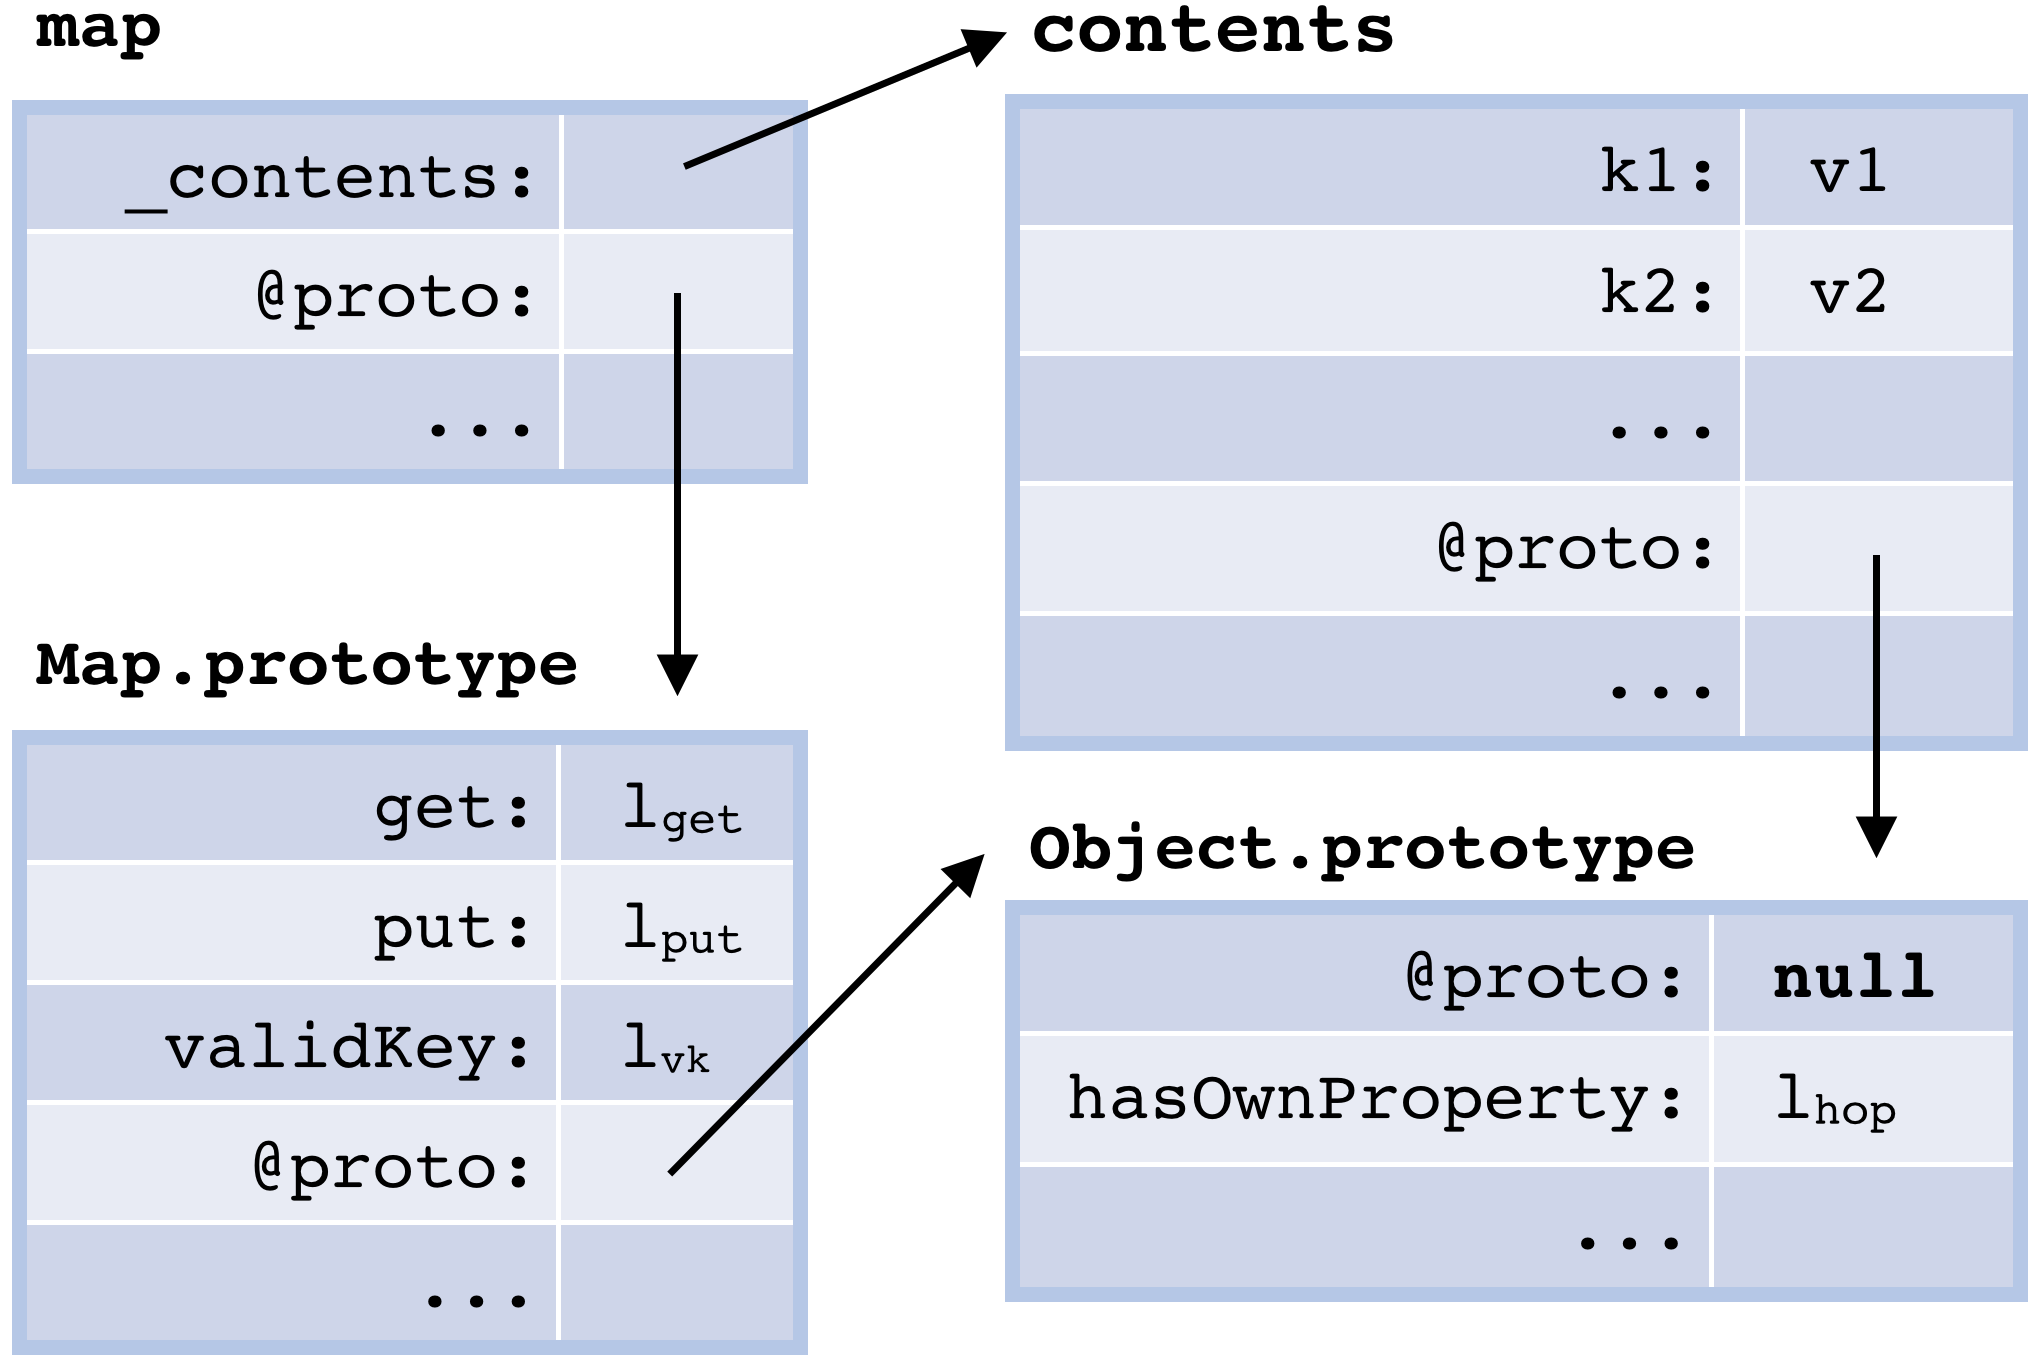
\includegraphics[width=1.2\textwidth]{figures/mapDiagram.png}
% \end{minipage}
%\vspace*{-0.3cm}
%\caption{JS map implementation (left) and example of a map library heap (right) \label{map:example}}
%\vspace*{-0.5cm}
%\end{figure}
%
%\myparagraph{Bug-finding}
%The map library implements a \emph{key-value map} as an object with property \jsinline|_contents|, denoting the object storing the map contents.  
%The named properties of \jsinline|_contents| and their value attributes correspond to the map keys and values, respectively.
%The functions \jsinline|get|, \jsinline|put|, and \jsinline|validKey| are to be shared between all map 
%objects. Therefore, they are defined in \jsinline|Map.prototype|, which is the prototype 
%of all objects created using \jsinline|Map| as a constructor (i.e.~using~\jsinline|new Map()|). 
%%
%Note that one can insert a key-value pair with \jsinline|"hasOwnProperty"| as a key into the map. 
%By doing this, \jsinline|"hasOwnProperty"| in the prototype chain of
%\jsinline|_contents| is overridden and subsequent calls to \jsinline|get| will fail. 
%Consider the following symbolic test:
%\begin{lstjsex}
%var s1 = __s(); var n1 = __n(); 
%var m = new Map();  m.put(s1, n1); var r = m.get(s1);  
%assert(n1 = r)
%\end{lstjsex}
%%
%The symbolic test above checks for a desired property of the library---if we were to put a key/value pair \jsinline|(k, v)| into the map, then we should be able to retrieve the value \jsinline|v| using the key \jsinline|k|. We can run \jilette on this test to reveal the bug discusses above. Indeed, \jilette generates
%the failing model: \jsinline|s1 = "hasOwnProperty"|. 
%
%This example also highlights how \jilette does not require 
%specialist knowledge, and can, therefore, be used by almost any JavaScript developer. 
%The annotation burden amounts to the creation of symbolic variables and the writing of assertions, remaining minimal and intuitive, in stark contrast with the standard annotation 
%burden of verification tools.
%
%%- Extensible Interpreter 
%% - an easy way to have more coverage 
%% - match the abstraction level of the generated code to the abstraction level of \rosette 
%
%\subsection{Supporting JavaScript Built-in Libraries}
%\label{builtins}
%
%JavaScript comes equipped with a rich runtime environment (described in Chapter 15 of the 
%ES5 standard~\cite{ecma}), which consists of \emph{built-in libraries} that support advanced manipulation of, for example, objects, arrays, strings, regular expressions, and dates. 
%In this section, we identify two important challenges related to supporting the symbolic execution of
%JavaScript programs that interact with built-in libraries and explain how we solve them in \jilette. 
%
%\JSComp models built-in library functions as \jsil procedures, which can be called from within the compiled JavaScript code. However, the current runtime environment of \JSComp does not support all built-in libraries described in the standard. In particular, it doesn't support regular expressions, parts of the String library that use regular expressions, parts of the Date library, and JSON objects. The partiality of \JSComp when it comes to supporting JavaScript built-in libraries 
%gives rise to the first challenge:  
%\begin{quote}
%\emph{Challenge 1:} \jilette should allow for modular addition of  
%implementations of built-in libraries not yet covered by \JSComp.  
%\end{quote}
%
%Most JavaScript library functions are described in the language standard in terms of 
%more elementary operations. For instance, operations on strings are often described in terms 
%of operations on the characters that comprise the string, and often involve loops (c.f. \jsinline|String.lastIndexOf|, Ch.15.5.4.8~\cite{ecma}).
%The \jsil implementations of the JavaScript built-in libraries follow the standard line-by-line, emphasising full adherence to the language standard. 
%However, for some of these built-in library functions, direct \rosette correspondents exist. 
%%
%In such cases, we argue that these correspondents should be used instead of the 
%functions provided by \JSComp, to minimise potential branching and looping on symbolic values. 
%Hence, we state the second challenge as follows: 
%\begin{quote}
%\emph{Challenge 2:} \jilette should prioritise native \rosette operations
%to the operations provided by \JSComp in the cases in which the native \rosette
%operations and JavaScript operations exactly match.
%\end{quote}
%
%\myparagraph{\rosette models of JavaScript built-in functions}
%To solve these two challenges, \jilette supports the on-the-fly extension of the \jsil interpreter 
%with \rosette implementations of JavaScript built-in functions, which we call \rosette \emph{models}. 
%Hence, every time the interpreter evaluates a procedure call, it first checks whether or 
%not it corresponds to a built-in function for which there is a \rosette model. If it does, 
%instead of executing the standard procedure call rule, the interpreter will instead 
%execute the appropriate \rosette model. 
%
%Below, we show a simplified \rosette model for the built-in \jsinline|String.prototype.replace|
%function~(see Ch.15.5.4.11~\cite{ecma}).
%This model uses the natively supported function \schemeinline|string-replace|, 
% taking advantage of \rosette reasoning capabilities.
%This example illustrates an important point about the difference between JavaScript and
%\rosette operations: \schemeinline|string-replace| works only with strings, but \jsinline|String.|\jsinline|prototype. |\jsinline|replace| can take arguments of any type that then get coerced to strings. Since \JSComp does not have an implementation of \jsinline|String.replace|, the \rosette model will report an error if it receives non-string arguments.
%\lstset{language=Scheme, numbers=none, backgroundcolor=\color{mygray}}
%\begin{lstlisting}
%(define (replace str from to)
%  (if (and (string? str) (string? from) (string? to))
%      (list (quote normal) (string-replace str from to #:all? #f))
%      (error "Unsupported call to String.prototype.replace")))
%\end{lstlisting}
%
%\myparagraph{Bug-finding with strings}
%By using the appropriate \rosette models for string operations, \jilette can find bugs in  
%non-trivial JavaScript programs that manipulate strings. For instance, consider 
%the following naive JavaScript implementation of a string sanitiser meant to remove 
%all occurrences of \emph{script tags} inside untrusted strings (for instance, those coming 
%from user input or untrusted servers).
%To this end, the programmer chooses to 
%replace all occurrences of the string \jsinline|"script"| in the string given 
%as input with \jsinline|"s"|. 
%\begin{lstjsex}
%function sanitise (str) { return str.replace("script", "s") }
%\end{lstjsex}
%Now, we can use \jilette to test if the sanitiser meets its purpose, that is, that all
%strings, after being sanitised, do not contain the substring \jsinline|"script"|:
%\begin{lstjsex}
%var s = sanitise(__s()); 
%var x = ! (s.contains("script")); d
%assert(x) 
%\end{lstjsex}
%\jilette will, in fact, be able to come up with a counter-model for this assertion. Concretely, this counter-model is \jsinline|s1 = "scriptcript"|. Despite its simplicity, this example illustrates the complexities underpinning the 
%design and implementation of robust string sanitisers, a commonly  
%used defense mechanism against XSS attacks~\cite{song}. 
% 
% 
%
 
 

%Furthermore, the \jsil language itself does not feature regular expressions or native arrays, 
%and has very few operators on strings. 
%This means that, for instance, more advanced operations on strings (such as 
%\jsinline|lastIndexOf|) need to be implemented as loops over the characters that comprise 
%the string. 
%






